\chapter{Resultados}
\label{sec:results}

Los siguientes resultados fueron producidos usando el generador de eventos \textsc{Pythia}, versión \verb|8.185|.

\section{Colisiones electrón-positrón en la resonancia $Z^0$}

En la simulación, cada energía de haz incidente es fijada a $45.6$ GeV, para reproducir la creación de la partícula de resonancia y sus subsecuentes decaimientos hadrónicos (descartando los leptónicos), es decir, $\ee\to Z^0\to \mbox{(hadrones)}$. Existe un conjunto limitado de datos experimentales que son relevantes para nuestro estudio.

\subsection{Tasa de ramificación de gluones en quarks bottom}

Los resultados experimentales para la tasa $\g_{\b\bbar}$ son mostrados en la tabla \ref{table:gbbMeasurements}.

\begin{table}[!h]
\caption{Datos experimentales para la tasaa de ramificación de gluones en $\b\bbar$.}\smallskip
\label{table:gbbMeasurements}
\centering 
\begin{tabular}{lcc}
\hline \hline  
\smallskip
Experimento & Ref. & $\g_{\b\bbar} (\pm(\text{estad.})\pm(\text{sist.})) (\%)$ \\ 
\hline
DELPHI & \cite{Abreu:1997nf} &  $0.21\pm0.11\pm0.09$ \\
ALEPH & \cite{Barate:1998vs} & $0.277\pm0.042\pm0.057$ \\
SLD & \cite{Abe:1999qg} & $0.307\pm0.071\pm0.066$ \\
DELPHI & \cite{Abreu:1999qh} & $0.33\pm0.10\pm0.08$ \\
OPAL & \cite{Abbiendi:2000zt} & $0.307\pm0.053\pm0.097$ \\
\end{tabular}
\end{table}

Los primeros tres valores fueron obtenidos estudiando pares secundarios de $\b\bbar$ de una muestra de cuatro jets de hadrones. El cuarto y el quinto valor provienen de estudios algo más recientes de la señal $Z\to\b\bbar\b\bbar$.

Una simulación de $10^7$ eventos fue llevada a cabo para cada una de la opciones. Los resultados se muestran en la tabla \ref{table:gbbResults}.


\begin{table}[!h]
\caption{Valores simulados de $\g_{\b\bbar}$ para cada opción.}\smallskip
\label{table:gbbResults}
\centering 
\begin{tabular}{cc}
\hline \hline  
\smallskip
Opción & $\g_{\b\bbar} (\pm(\text{estad.}) (\%)$ \\ 
\hline
1 &  $0.397\pm0.002$ \\
2 &  $0.527\pm0.002$ \\
3 &  $1.106\pm0.003$ \\
4 &  $0.407\pm0.002$ \\
5 &  $0.384\pm0.002$ \\
6 &  $0.504\pm0.002$ \\
7 &  $1.083\pm0.003$ \\
8 &  $0.389\pm0.002$ \\

\end{tabular}
\end{table}


Como es de esperarse, la tabla refleja la descripción de las opciones. La opción 2 da una tasa más alta que la opción por defecto, ya que añade el término de masa que corrige el comportamiento en la región umbral, mientras que la opción 3 es aún mayor, debido al denominador ($1-\delta$). La opción 4 provee un valor cercano al dado por la opción 1; el acrecentamiento presente en la región umbral, se ve aproximadamente cancelado por la supresión presente a masas altas.

La producción de $\b\bbar$ como función de la masa invariante del par es mostrada en la figura \ref{fig:QMass}.


\begin{figure}[h]
\centering
\caption[Producción de pares de quarks bottom (cuatro opciones).]{Producción de pares bottom-antibottom como función de la masa invariante. Opciones de \textsc{Pythia}: por defecto (sólida), 2 (líneas), 3 (puntos) y 4 (líneas y puntos).}
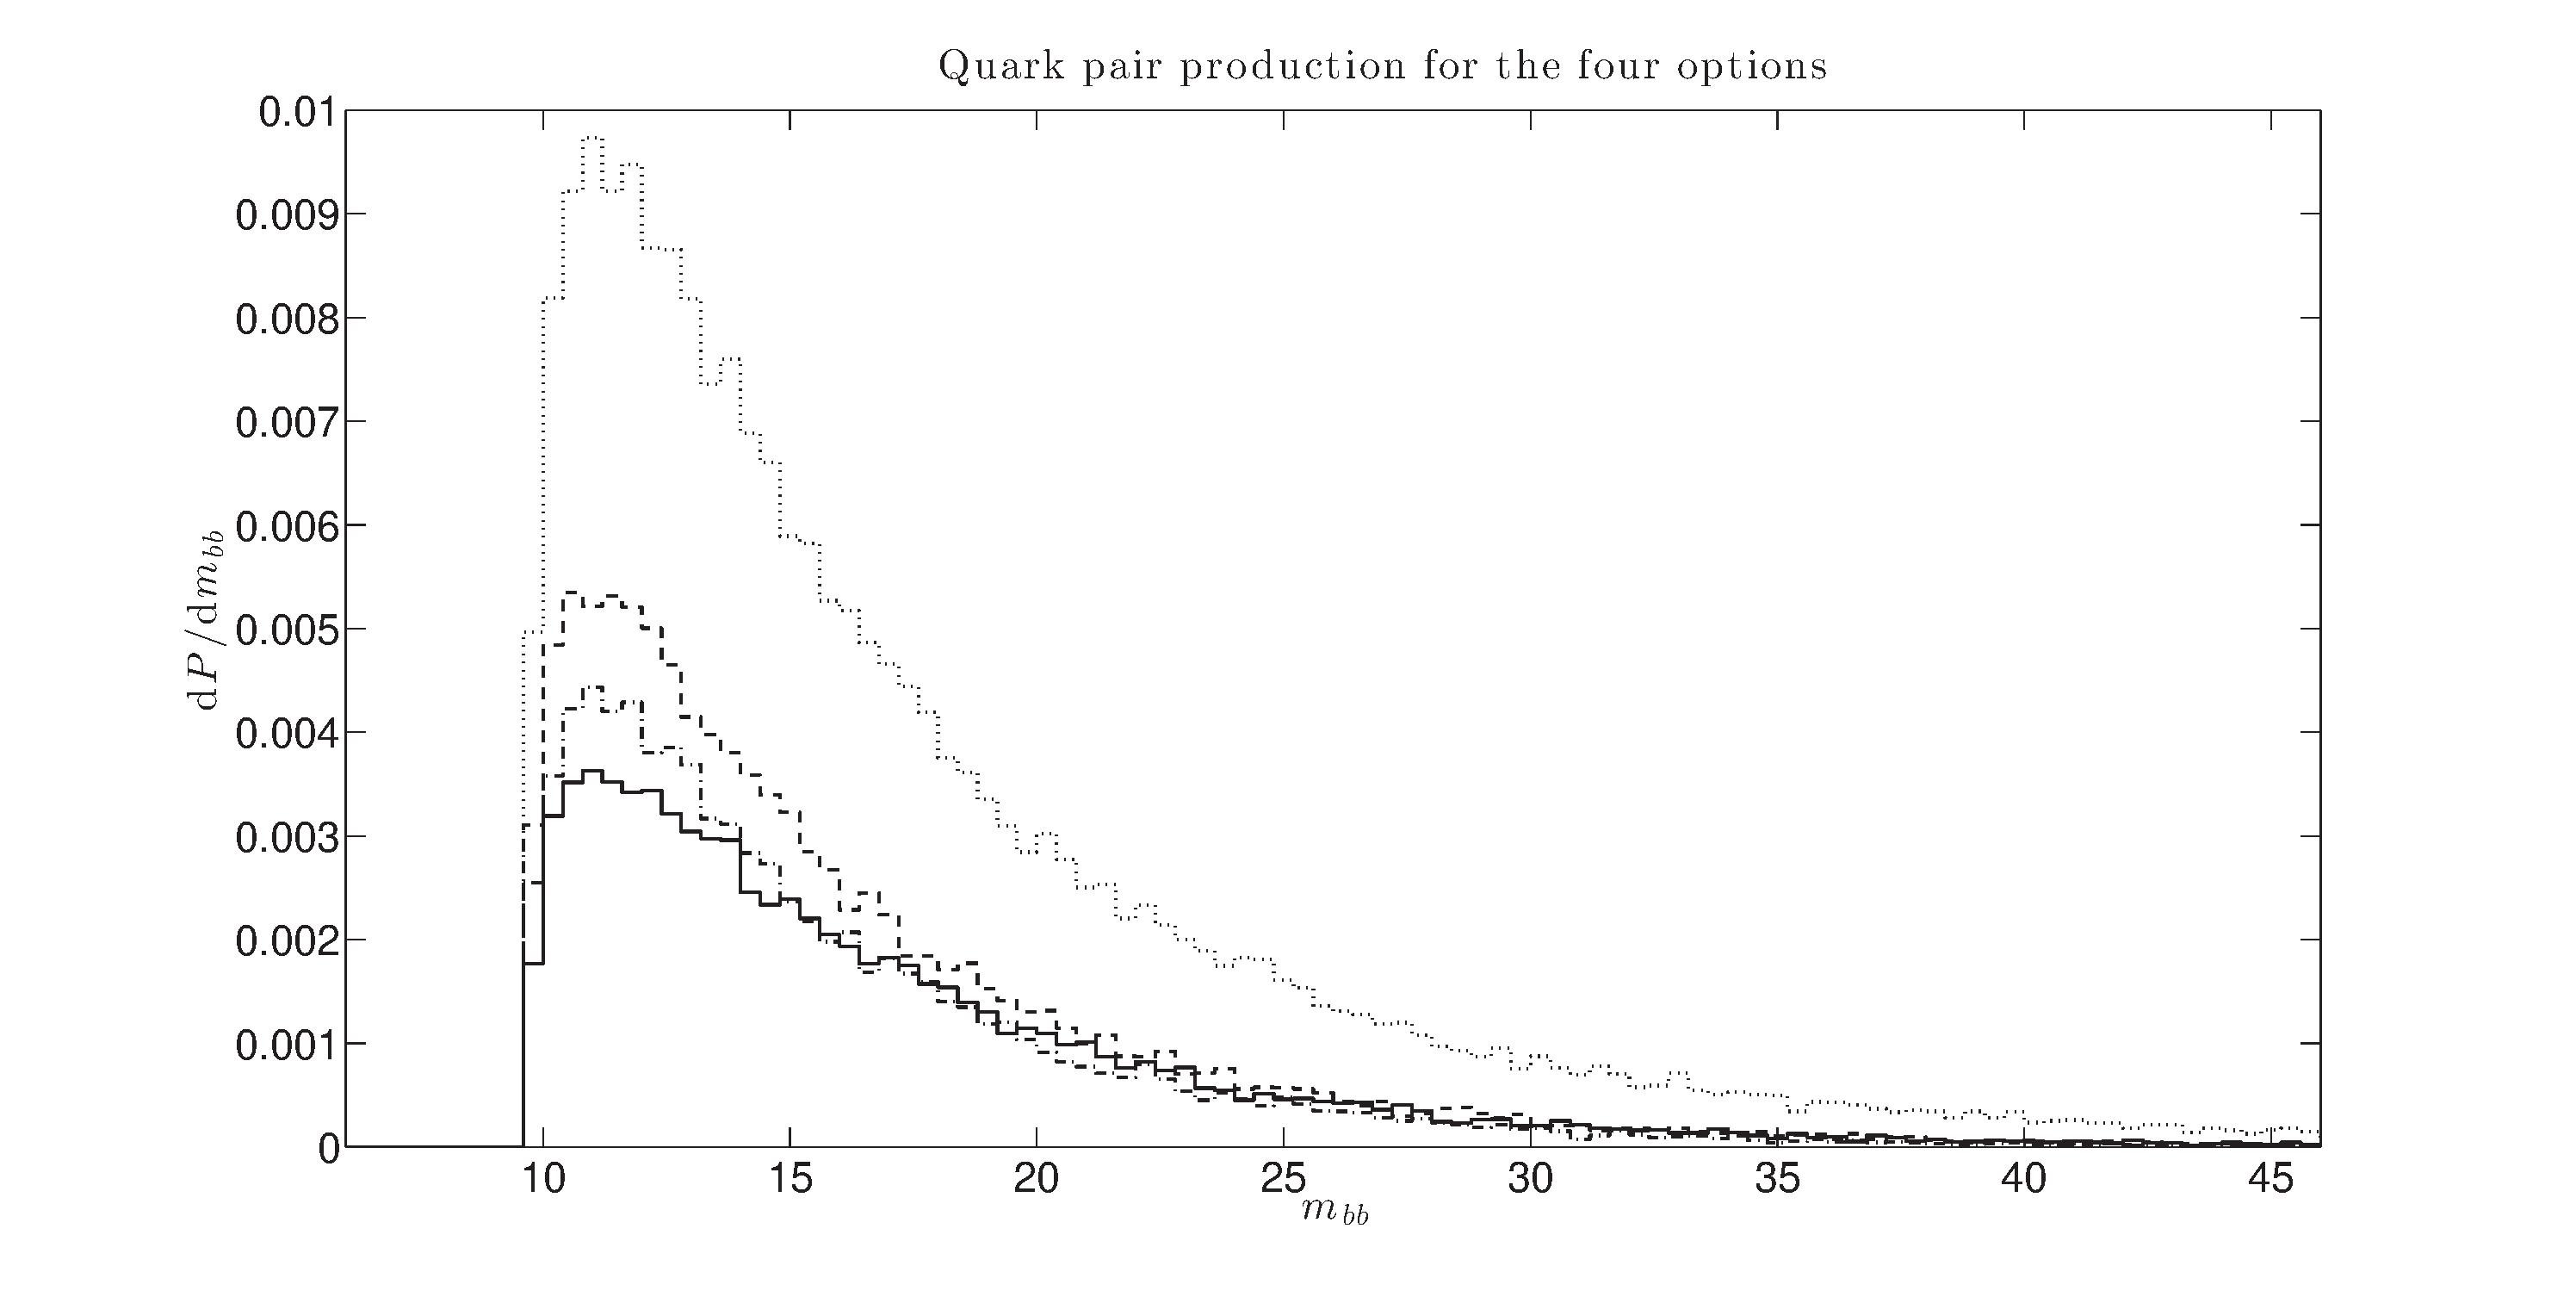
\includegraphics[width=15cm]{QMass}
\label{fig:QMass}
\end{figure}



Las características importantes de las opciones 1-4, discutidas en \ref{subsubsec:PythiaAlg}, están presentes en este gráfico. La opción 3 representa el caso extremo. La compensación entre el acrecentamiento en la zona umbral y la supresión a masas altas es visible para la opción 4. Esta compensación corrige el valor de la tasa total (área bajo la curva) a un valor similar al dado por la opción 1. En principio, no hay ninguna razón para esperar que estos dos efectos se compensaran tan cercanamente en la tasa total. La opción 2 presenta una producción visiblemente mayor que la opción 1 en la zona umbral de producción.

Las tasas dadas por las opciones que usan $m^2$ como variable de evolución (5-8) conllevan a una tasa ligeramente menor que las dadas por las primeras 4 opciones, alrededor de 5\% menos.

Los valores dados por las opciones 1, 4, 5, 6 y 8 caen dentro del error total de las últimas tres referencias en la tabla \ref{table:gbbMeasurements}. El valor dado por la opción 2 está por poco fuera de los errores, pero aún dentro de dos desviaciones estándar. Las opciones 3 y 7 no parecieran resproducir los datos experimentales, ya que se encuentran lejanamente fuera del límite superior indicado por todas las mediciones.

Las discrepancias pueden estar relacionadas a la masa desnuda del quark bottom, una cantidad que no puede ser medida directamente. Usando una masa $m_\b$ más alta que la dada por defecto, las tasas simuladas se reducirían, acercándose más a los resultados experimentales. Además, tomando en cuenta los errores sistemáticos mostrados en la tabla \ref{table:gbbMeasurements} y la dispersión de los valores, podemos notar que se trata de una medición complicada.

\subsection{El espectro de la fracción de energía de los mesones $\D^{*\pm}$}

Vamos a estudiar ahora la producción de mesones $\D^{*\pm}$ como función de la fracción de energía $X_E$. La colaboración ALEPH tiene mediciones para esto en \cite{Barate:1999bg}. El espectro total es tomado como la suma de tres componentes: mesones provenientes de charms primarios, de bottoms primarios y de quarks pesados secundarios, es decir, provenientes de ramificaciones a partir de gluones.

\begin{figure}[h]
\centering
\caption[Espectro de la fracción de energía de los mesones $\D^{*\pm}$.]{Distribución de la fracción de energía para los mesones  $\D^{*\pm}$. Los puntos con barras de error son las mediciones de ALEPH  y la línea sólida corresponde a la simulación de \textsc{Pythia}, con las contribuciones correspondientes de: $\b\bbar$ (puntos), $\c\cbar$ (líneas) y ramificaciones de gluón (líneas y puntos).}
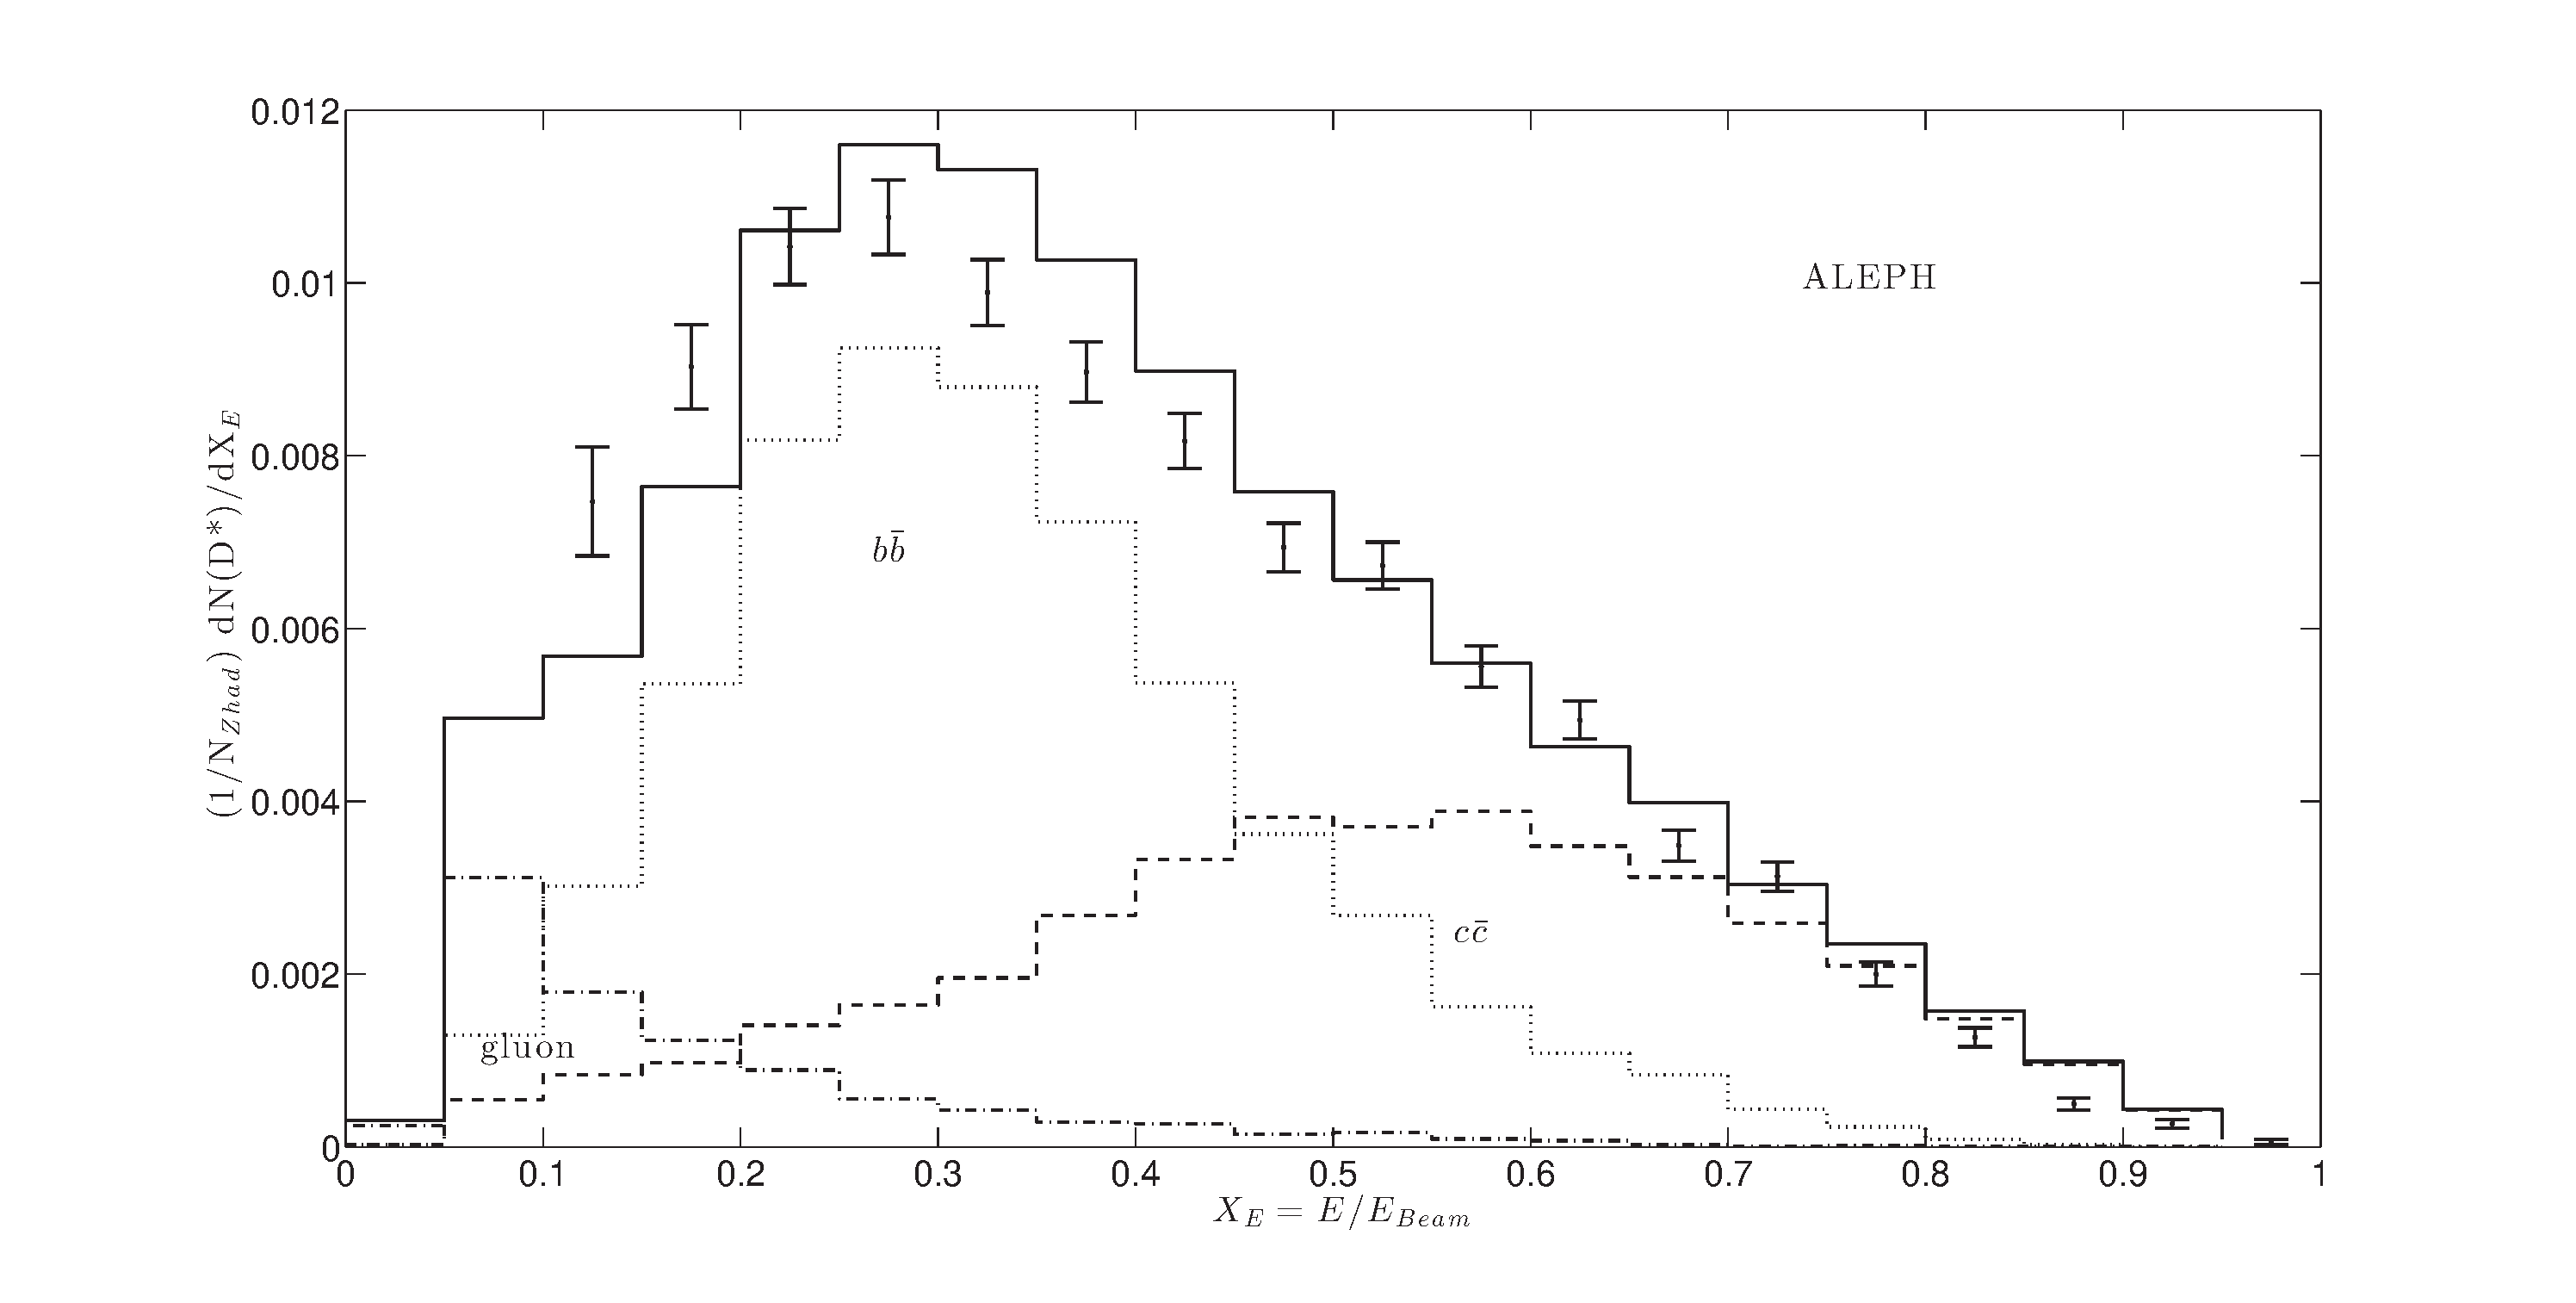
\includegraphics[width=15cm]{DStarOp1Thesis}
\label{fig:ALEPHPythia1}
\end{figure}



En gráfico en la figura \ref{fig:ALEPHPythia1} muestra que las mediciones de ALEPH y la simulación de \textsc{Pythia} (opción 1) con sus componentes. Podemos ver que la contribución principal de la ramificación de gluones sucede a fracciones de energía bajas, lo que se debe al hecho de que los quarks secundarios son producidos al menos en una tercera ramificación, partiendo desde el $Z^0$ (como en la figura \ref{fig:PrimSecQuarks}), cuando ya la energía ha sido distribuída en varios productos. De este modo, el impacto de las opciones será a fracciones de energía bajas. La figura también sugiere la necesidad de una corrección a energías bajas, incluso para las contribuciones de $\b\bbar$ y $\c\cbar$ primarios. Además, la simulación presenta un exceso justo después del pico cercano a $0.3$. Para valores medianos y altos de $X_E$, la simulación y los experimentos concuerdan en buena medida.

La figura \ref{fig:GluonDStar} muestra los casos extremos para la contribución de gluones: opciones 1 y 3. La última presenta valores al menos dos veces mayores que la primera en cada casilla del histograma. Las distribuciones para las opciones 2 y 4 (que no se muestran) dan valores intermedios.

\begin{figure}[h]
\centering
\caption[Contribución de los gluones a la producción de $\D^{*\pm}$ en dos casos extremos.]{Casos extremos de la producción de $\D^{*}$ a partir de gluones. Opciones de \textsc{Pythia} 1 (sólida) y 3 (punteada).}
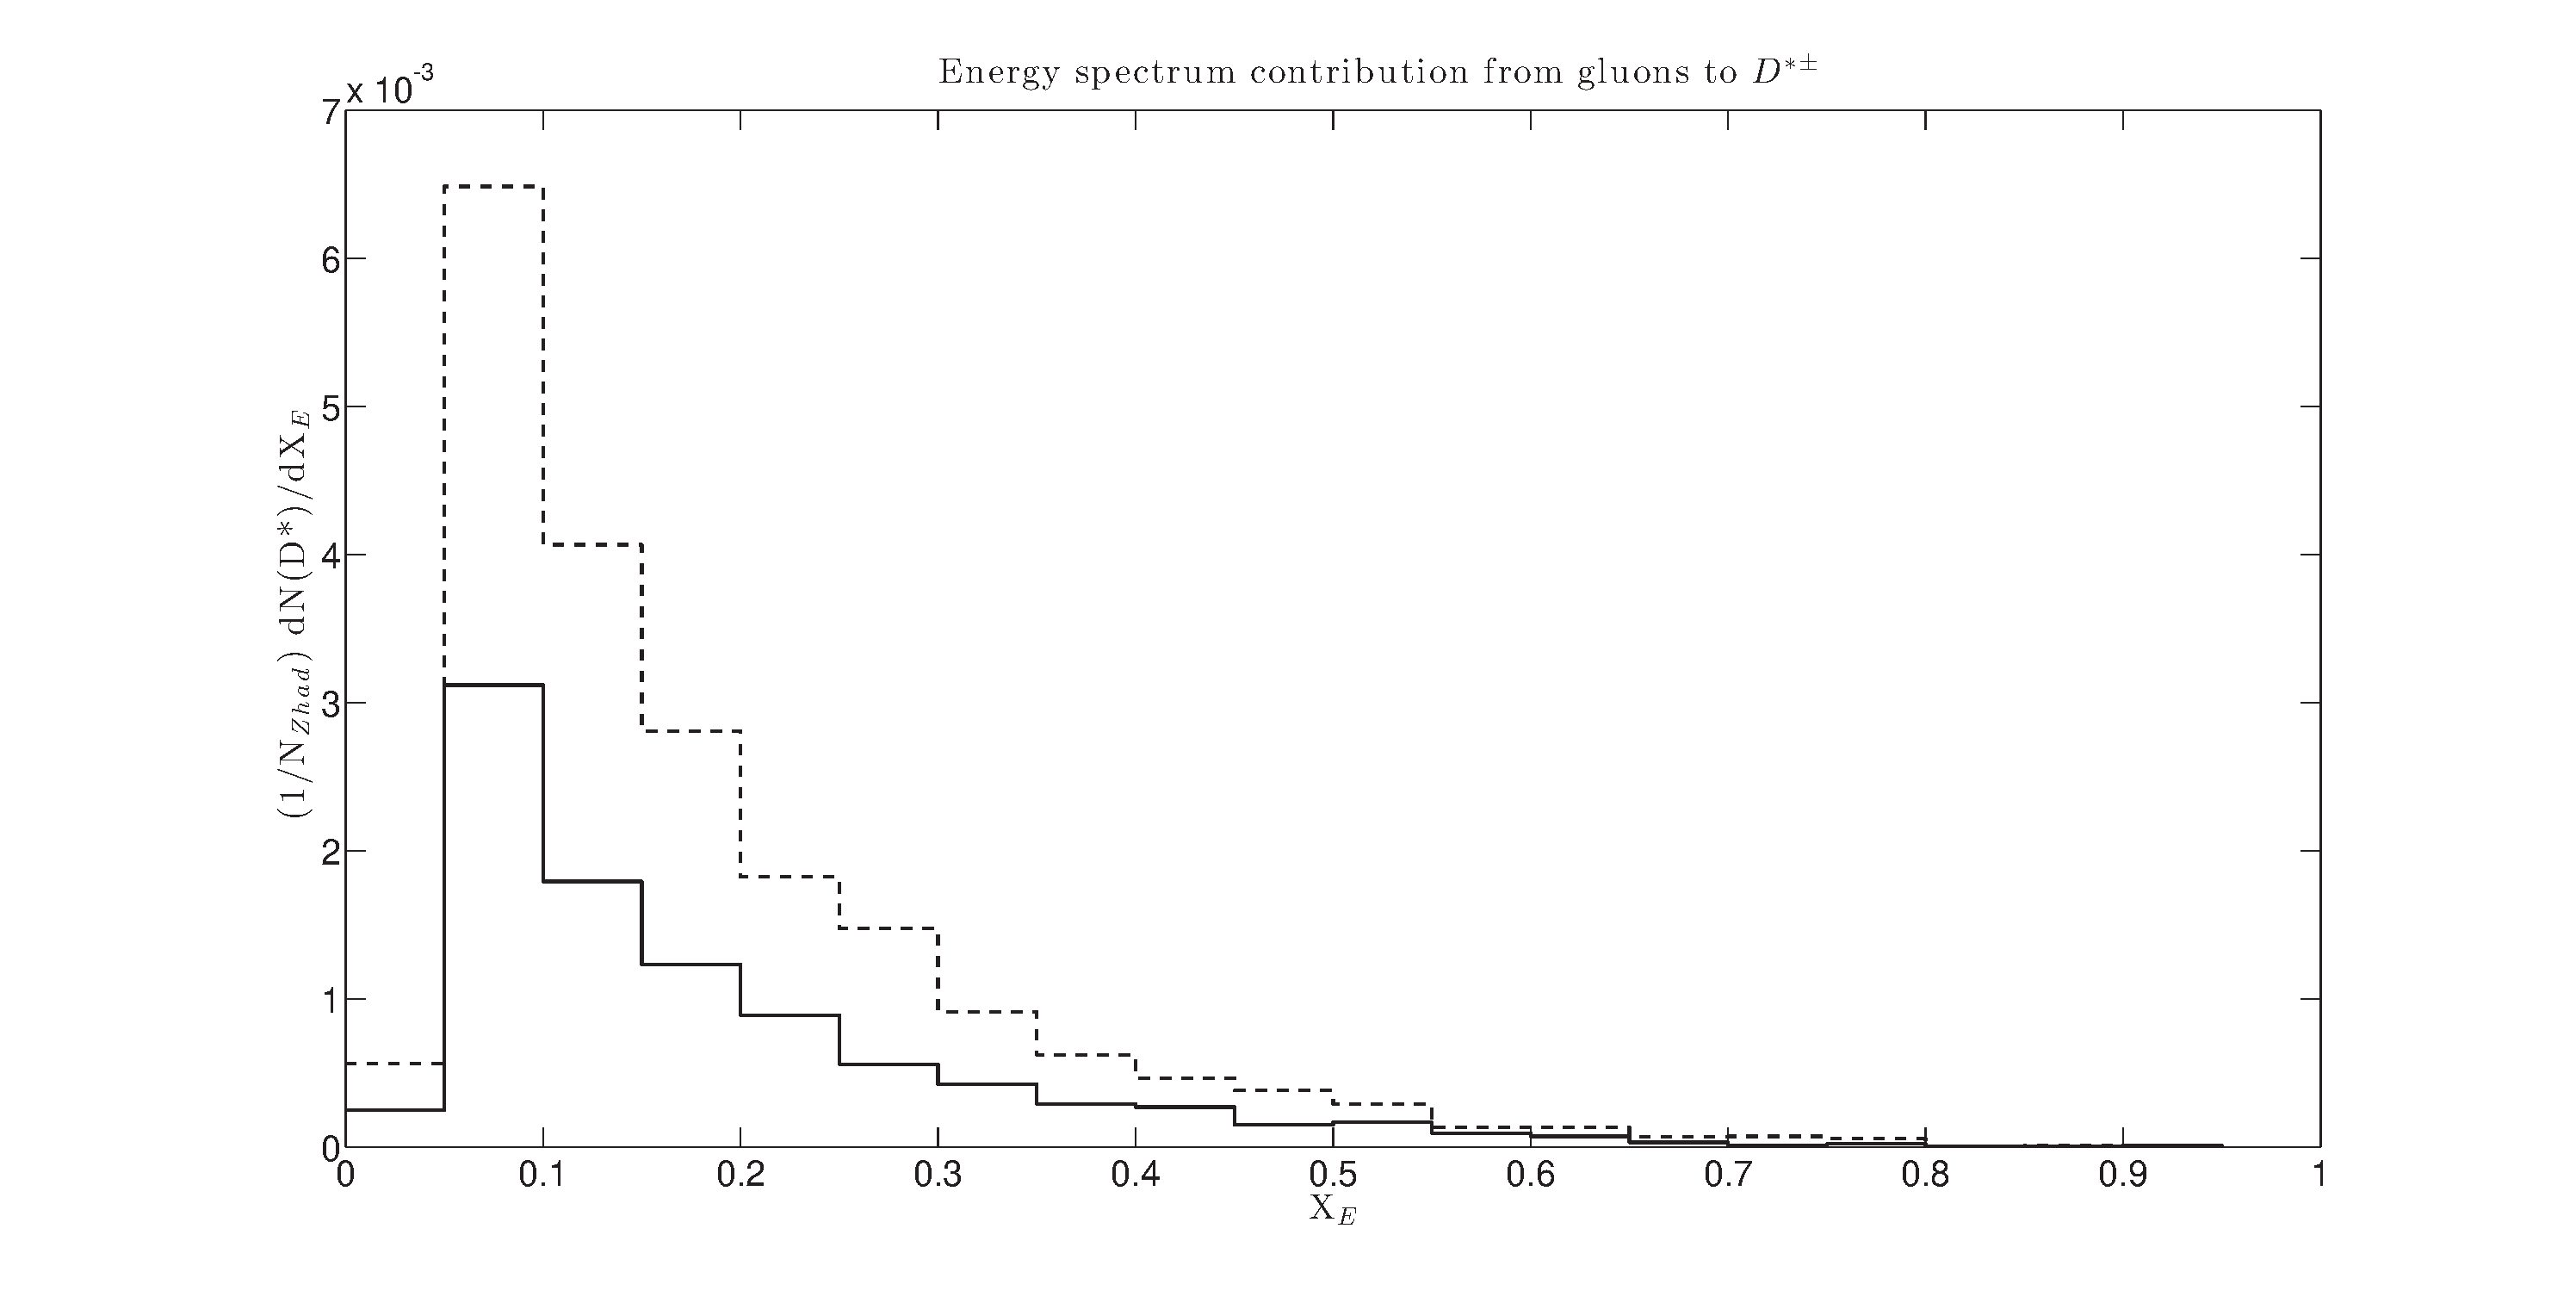
\includegraphics[width=15cm]{GluonDStarThesis}
\label{fig:GluonDStar}
\end{figure}

Para comparar las cuatro opciones con los datos experimentales, la figura \ref{fig:DStarOp} muestra las distribuciones completas y las mediciones de ALEPH. El aumento de producción a bajas energías es evidente para las opciones que no son por defecto, donde las simulaciones se acercan más a los valores experimentales. El exceso cercano al pico está todavía presente y ligeramente aumentado. A altas energías, el decaimiento no muestra diferencias significativas con respecto a la opción por defecto (debido a que en esta zona la contribución secundaria es despreciable) y siguen aproximadamente el comportamiento de los datos.

\begin{figure}[!h]
\centering
\caption[Espectro de la fracción de energía de $\D^{*\pm}$. Simulación y datos comparados.]{Espectro de la fracción de energía de $\D^{*\pm}$. Datos de ALEPH (puntos con barras de error) y las opciones de \textsc{Pythia}: por defecto (sólida), 2 (puntos), 3 (líneas) y 4 (líneas y puntos).}
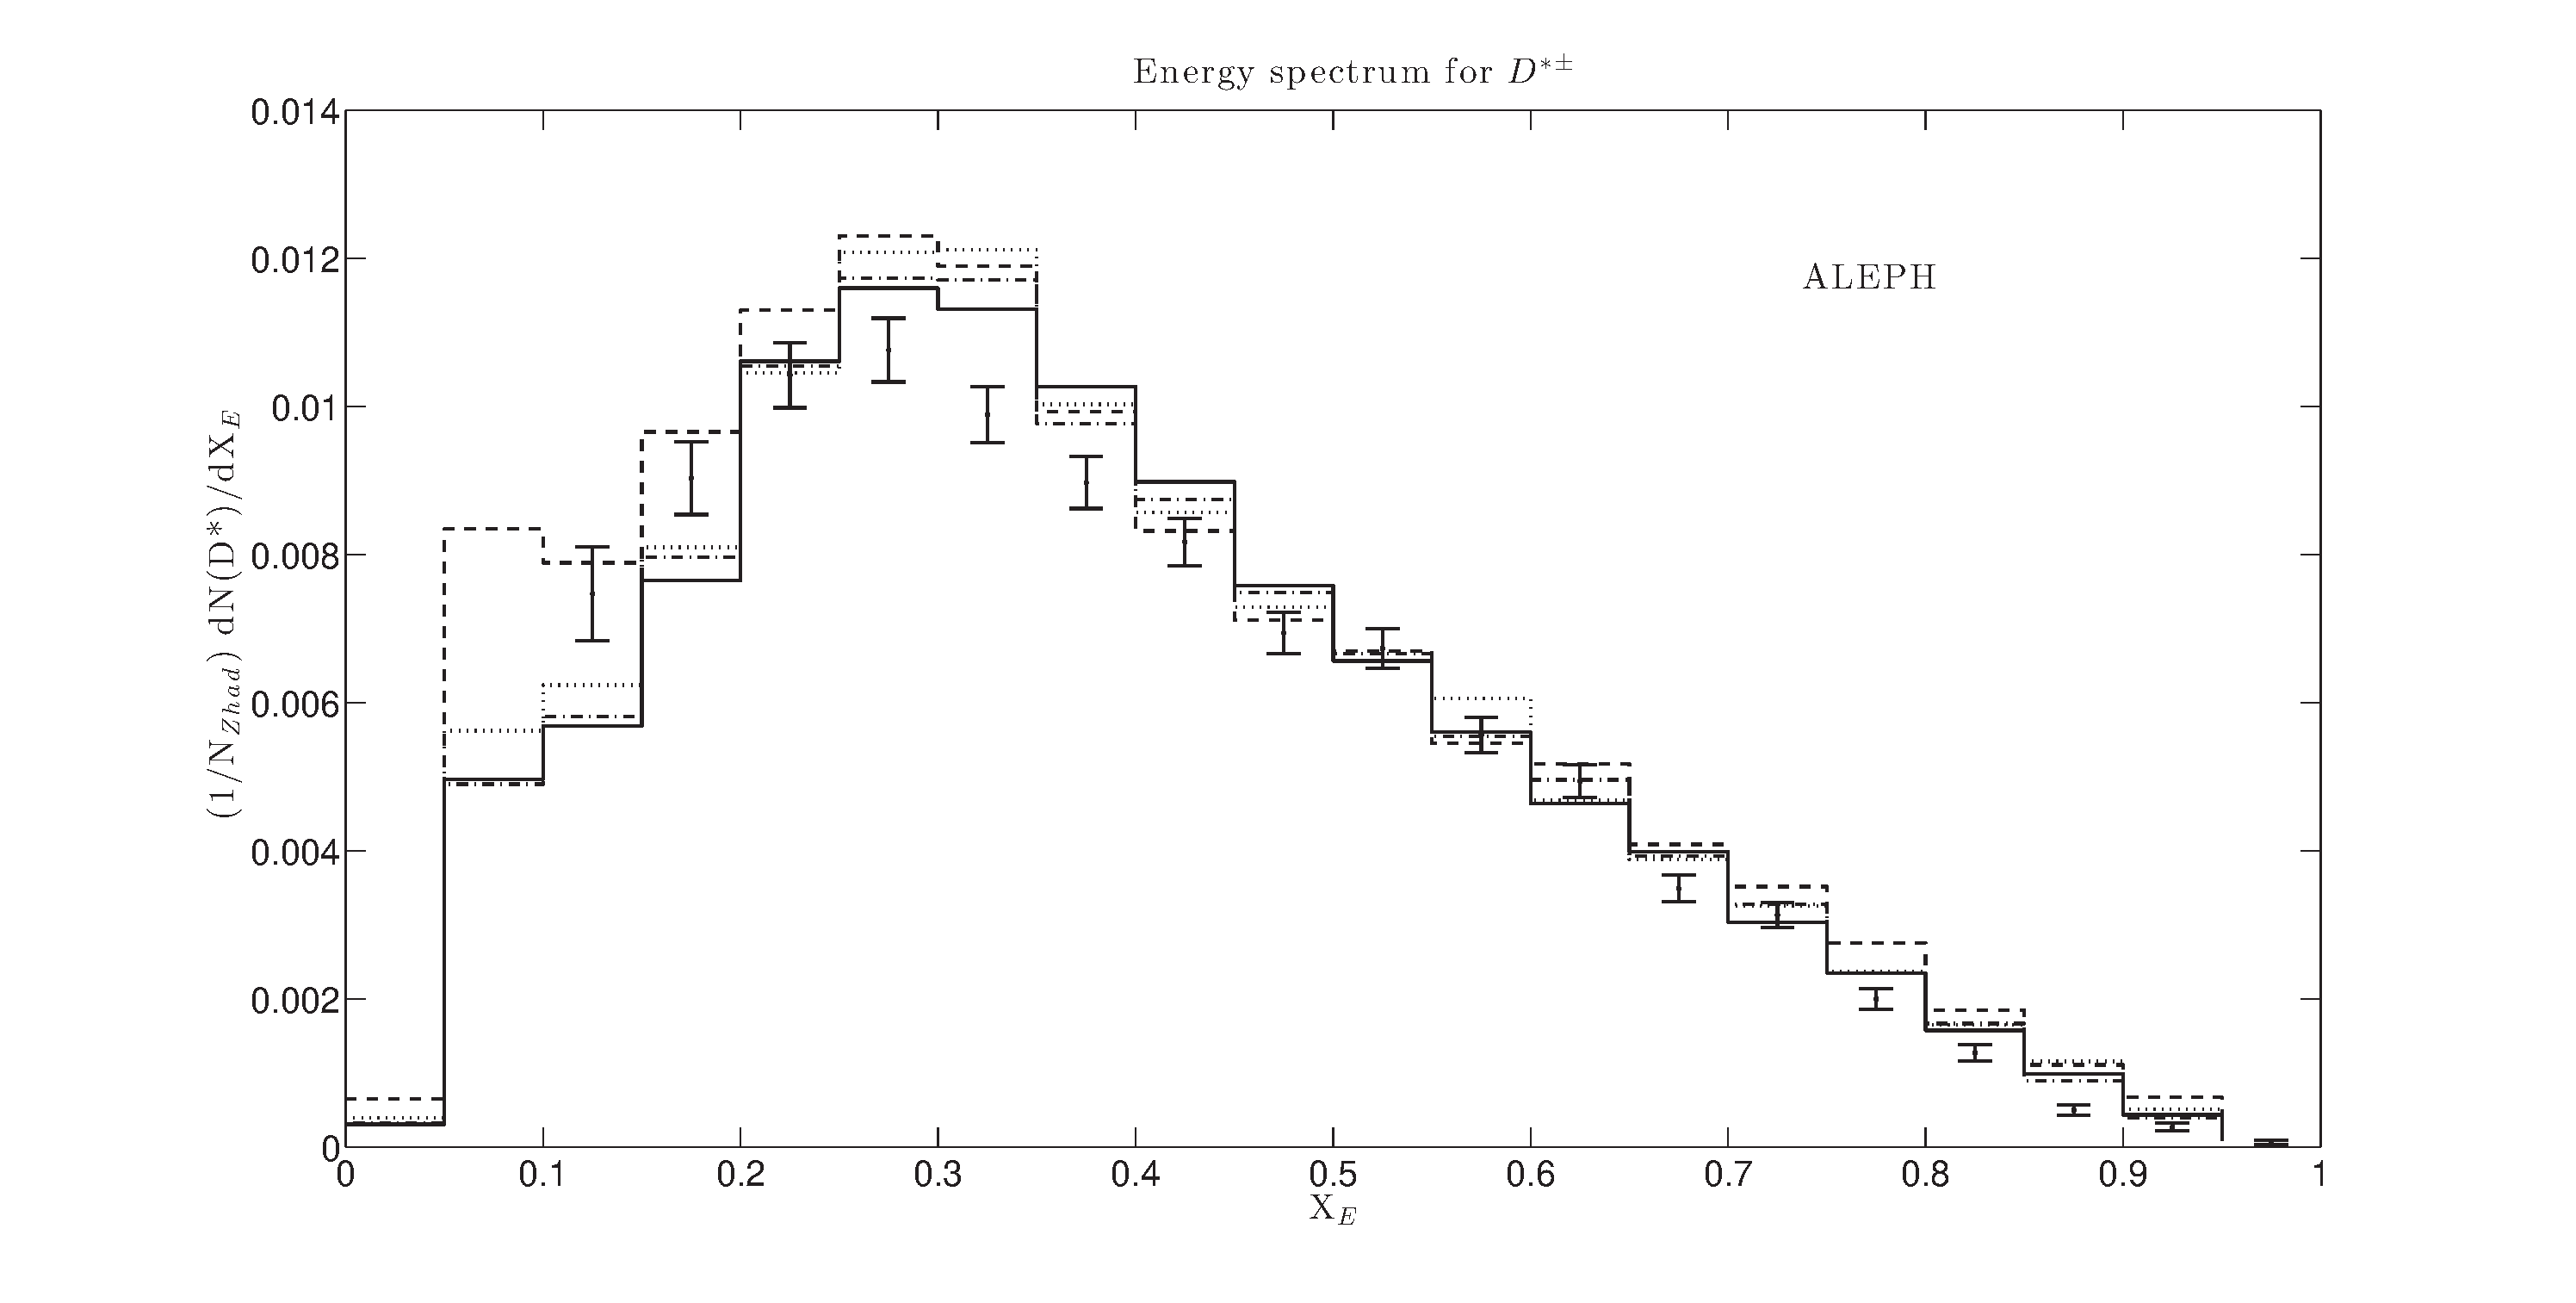
\includegraphics[width=15cm]{DStarOpThesis}
\label{fig:DStarOp}
\end{figure}

En este contexto, la opción 3 parece un buen candidato, debido a que corrige (con algo de precisión) la producción de mesones $\D^*$ a bajas energías. Para la región justo después del pico, el aumento puede ser mayor al deseado, pero aún así los datos en su totalidad son más cercanos a esta opción.

Debido a su carácter no-perturbativo, el decaimiento de mesones es un fenómeno que no se entiende completamente. Un modelado algo diferente del decaimiento $\B\to D$ pudiera correr algunos eventos después del pico a más bajas energías, para ajustarse mejor a los datos experimentales en ambas regiones, sin requerir una tasa $\g\to\b\bbar$ mayor. De esta manera, este estudio no puede concluir definitivamente sobre esta desviación.

\section{Colisiones protón-protón a 7000 GeV}

Tornando ahora al tema de las colisiones hadrónicas, estudiaremos las correlaciones entre pares de hadrones $\B$. Eventos con un par son clasificados de acuerdo a PC, FE y GS. Eventos con más pares son clasificados como mezclados.

Una simulación de $5\times10^6$ eventos fue llevada a cabo para cada opción. Fueron seleccionados para el análisis eventos con dos mesones $\B$, cada uno con un momentum transverso mayor a 15 GeV. Un corte inferior para el momentum transverso del proceso duro de 15 GeV también fue impuesto; este criterio es necesario debido a que eventos con $\pT$ más bajo son producidos en mayor cantidad, pero el número de eventos seleccionados decrece para valores menores de 20 GeV, como se puede ver en la figura \ref{fig:accepted}. Allí, sólo alrededor del 1\% de los eventos son seleccionados para el análisis. Un corte aún más bajo incrementaría tal ``ineficiencia'', seleccionando sólo unos pocos más eventos en comparación con el total generado.

\begin{figure}[h]
\centering
\caption[Eventos generados y aceptados en colisiones hadrónicas.]{Eventos generados (sólida) y aceptados (punteada) como función del momentum transverso del proceso.}
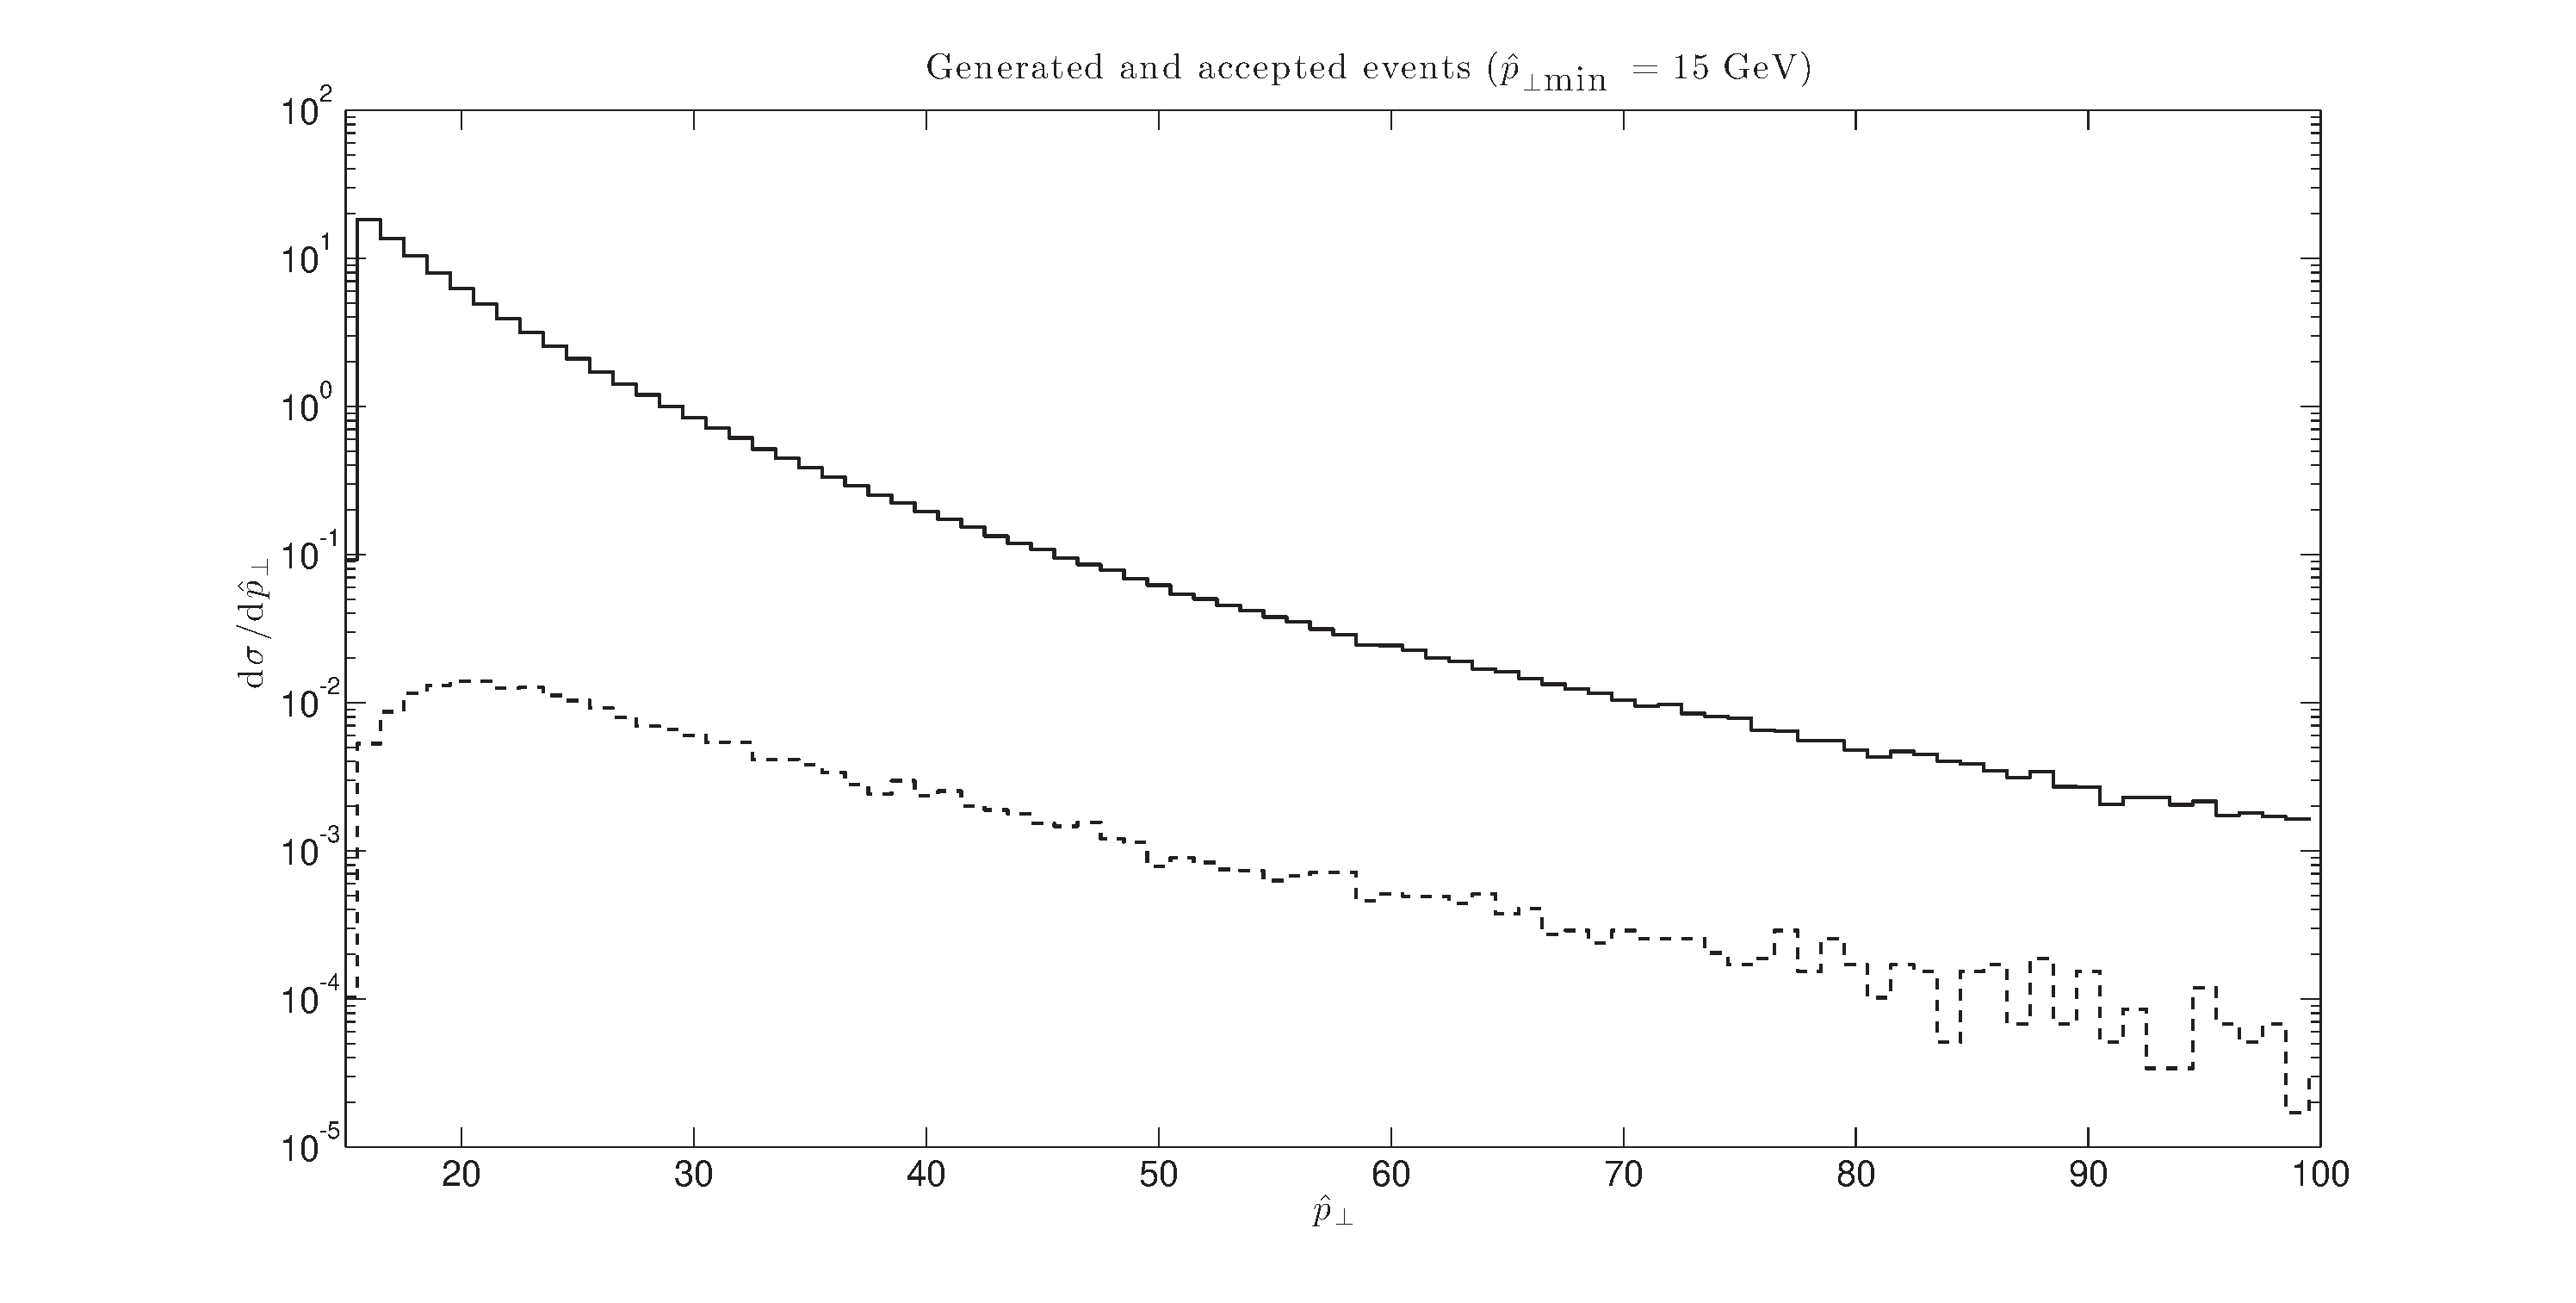
\includegraphics[width=15cm]{Accepted}
\label{fig:accepted}
\end{figure}

\subsection{Separaciones azimutales angulares}

La variación del ángulo azimutal es una buena medida de la separación de dos mesones $\B$, debido a que es un invariante de Lorentz bajo boosts a lo largo del eje de colisión ($z$). La diferencia $\Delta \varphi$  es medida en el plano perpendicular al eje $z$. La figura \ref{fig:BBPhiOp1}  muestra la producción de pares de mesones bottom en términos de la separación angular azimutal, para la opción 1.

\begin{figure}[!h]
\centering
\caption[Separación angular azimutal de pares de mesones $\B$. Opción por defecto de \textsc{Pythia}.]{Separación angular azimutal de pares de mesones $\B$ usando la opción por defecto de \textsc{Pythia} incluyendo las cuatro fuentes de producción.}
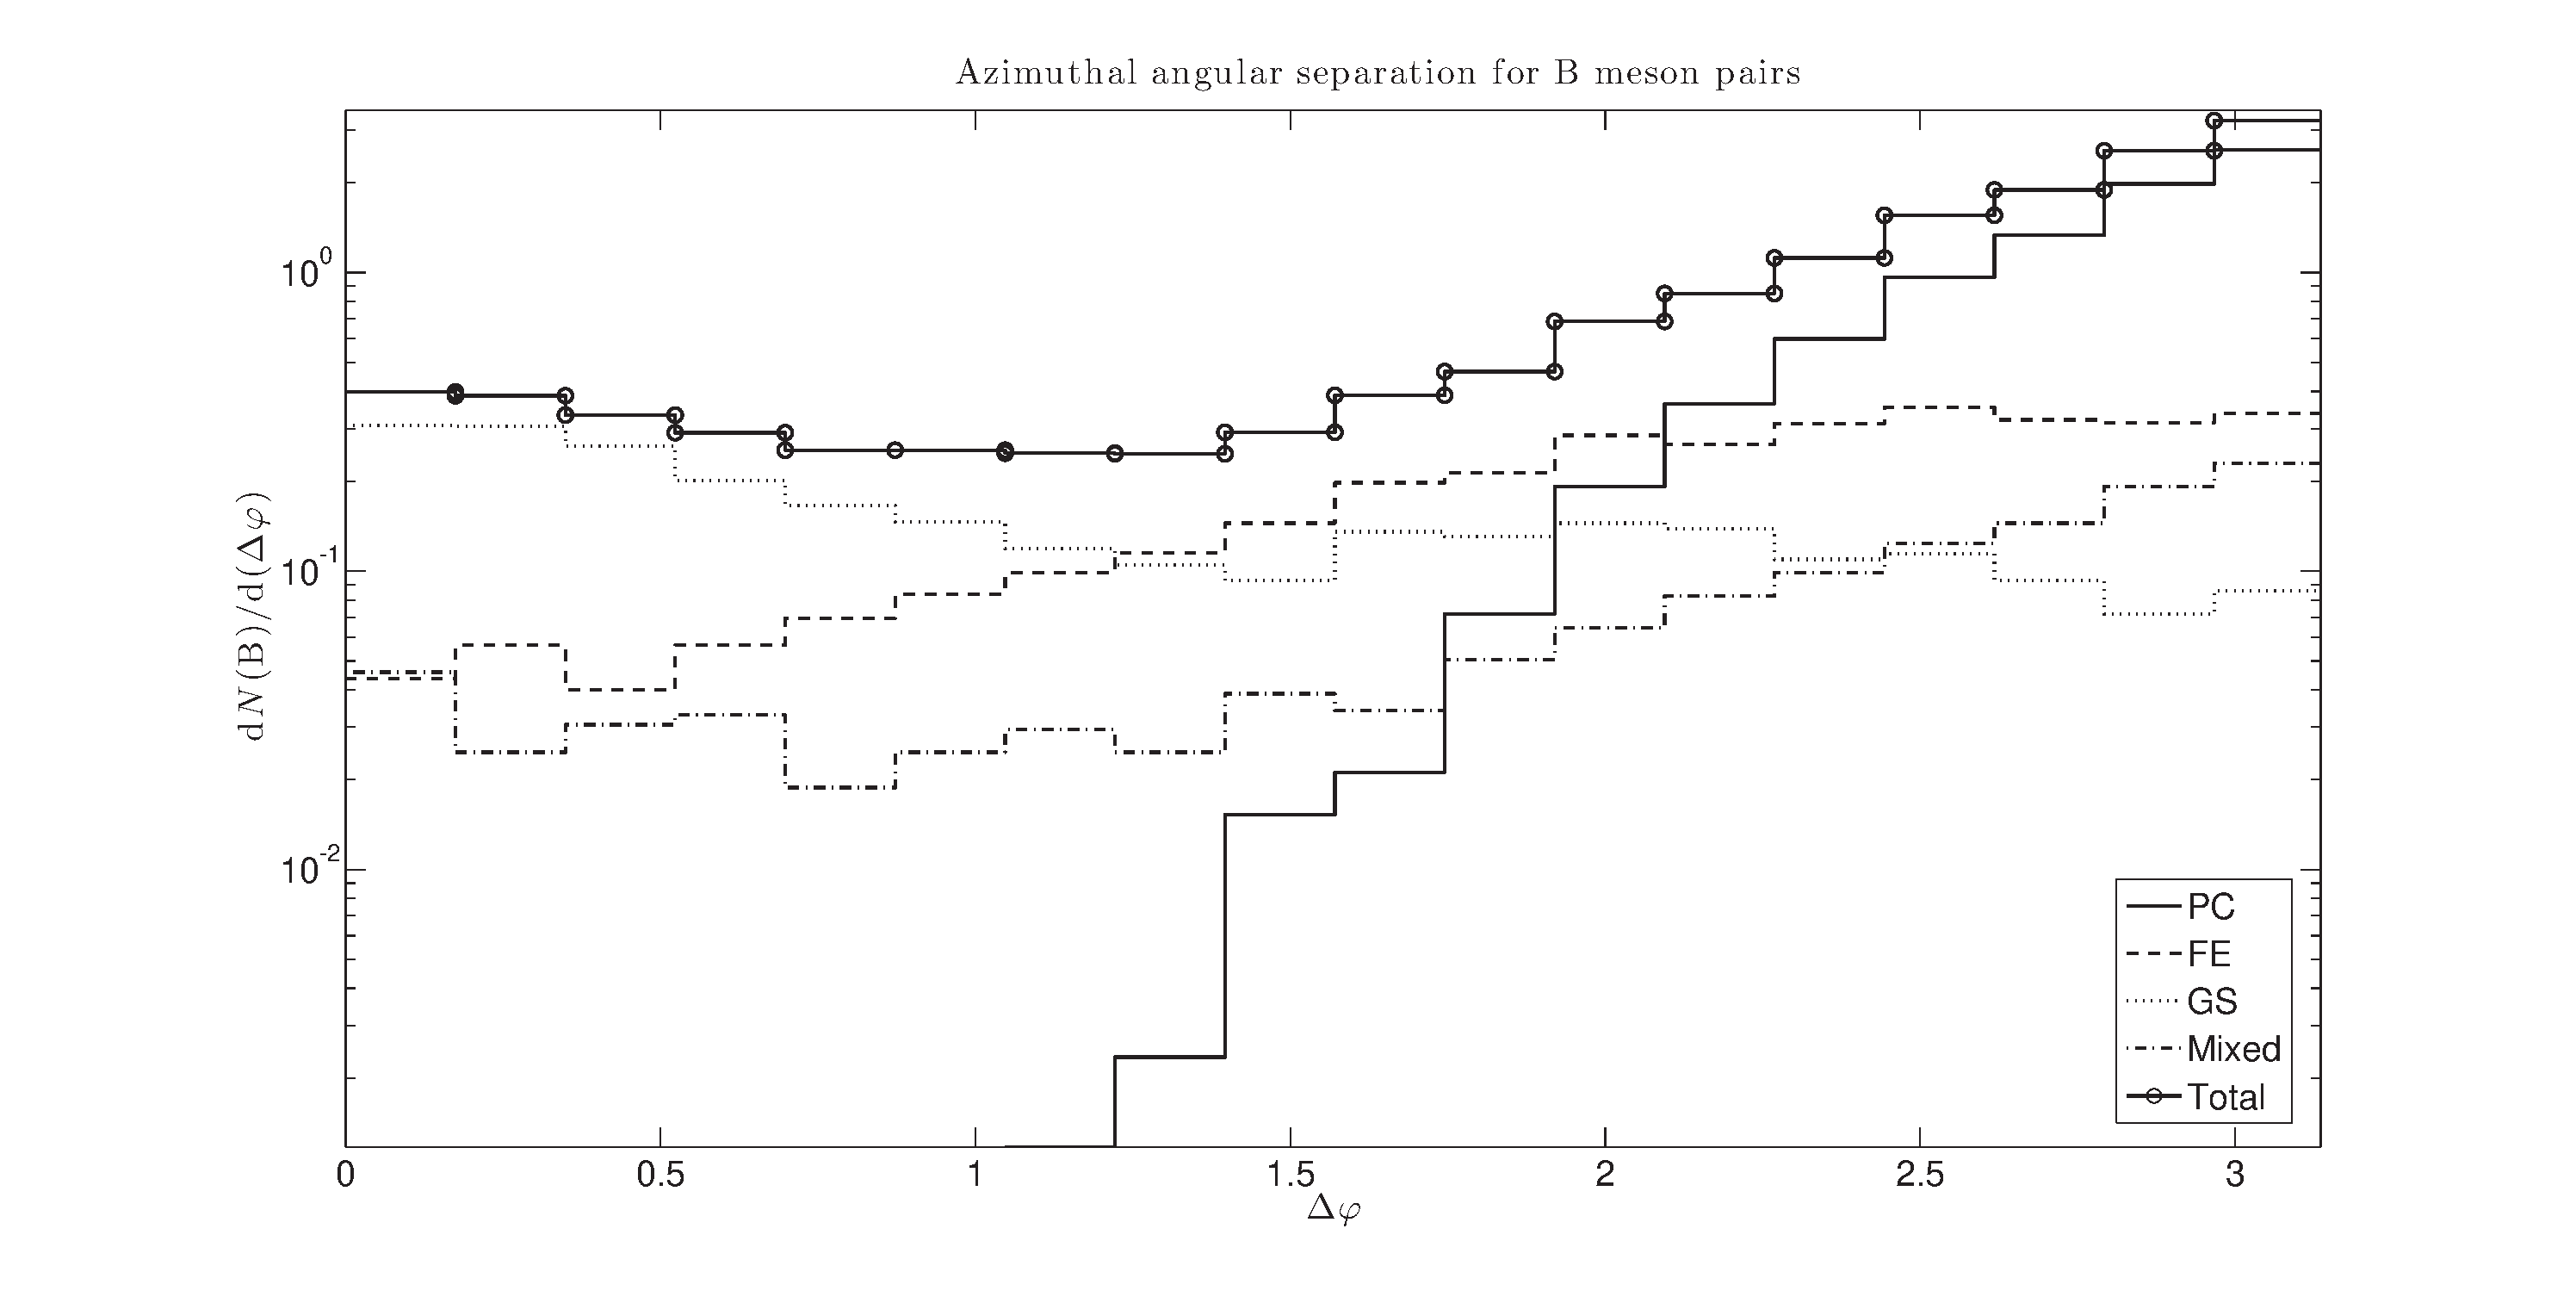
\includegraphics[width=15cm]{BBPhiOp1}
\label{fig:BBPhiOp1}
\end{figure}
Varios rasgos de las correlaciones en los mecanismos de producción son visibles: PC muestra un pico a ángulos altos, debido a que los pares son creados en el proceso duro y tienden a producir quarks en sentidos opuestos, mientras que GS contribuye mayormente en la región de poca abertura. Pares creados a partir de FE están menos anticorrelacionados que los provenientes de PC. Los mesones $\B$ mezclados muestran una distribución angular homogénea, ya que no hay una relación particular entre los mesones provenientes de ramificaciones de gluones distintas.

La variación de las opciones de \textsc{Pythia} es mostrada en la figura \ref{fig:BBPhi4Op}.

\begin{figure}[!h]
\centering
\caption[Separación angular de pares de mesones $\B$. Cuatro opciones de \textsc{Pythia}.]{Separación angular azimutal de pares de mesones $\B$ usando las opciones de \textsc{Pythia} 1 (sólida), 2 (líneas), 3 (puntos) y 4 (líneas y puntos).}
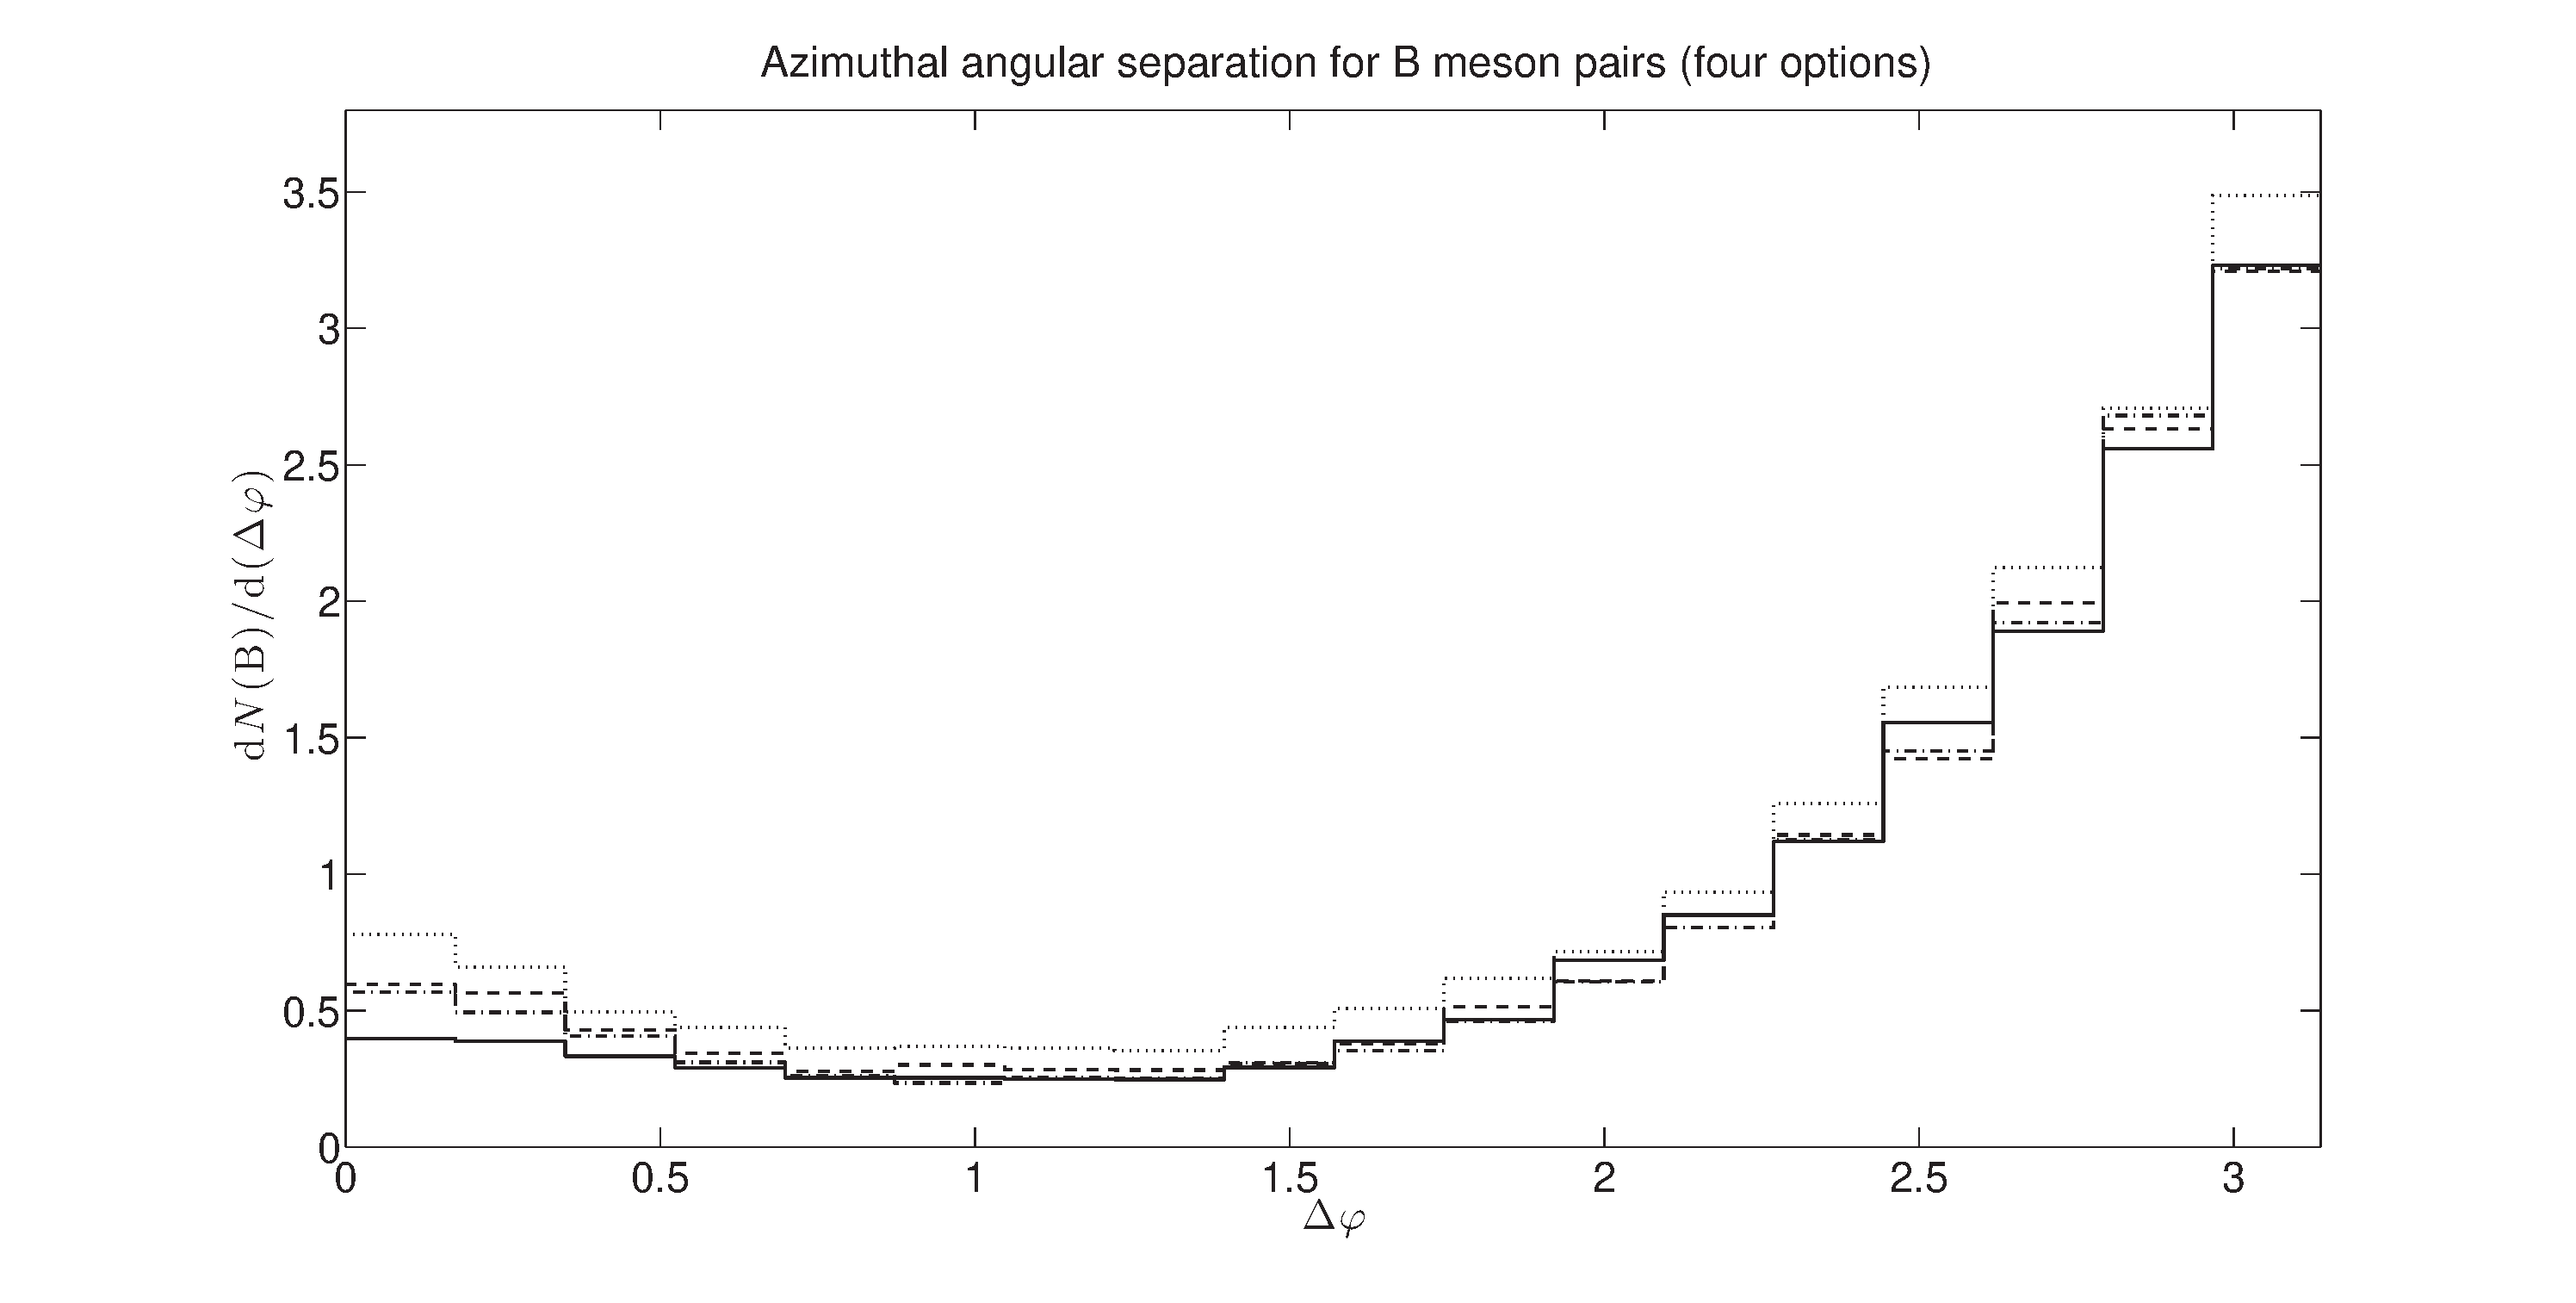
\includegraphics[width=15cm]{BBPhi4Op}
\label{fig:BBPhi4Op}
\end{figure}
De manera similar al caso discutido en la sección previa, los dos casos extremos (superior e inferior) a ángulos azimutales bajos están dados por la opciones 3 y 1, donde la ramificación de gluones es dominante. Las opciones 2 y 4 son intermedias en esta región.

\subsection{Rapideces relativas}

La rapidez, definida como

$$
y =\frac12 \ln \frac{E+p_z}{E-p_z},
$$
es una medida de la separación de la partícula al eje $z$. De hecho, está relacionada al ángulo polar (entre la partícula y el eje $z$). Se puede mostrar que la diferencia $\Delta y \equiv y_2 - y_1$ es invariante bajo un boost a lo largo del eje $z$.

En gráfico en la figura \ref{fig:BBYOp1} muestra la producción de pares de mesones $\B$ como una función de las rapideces relativas $\Delta y$, simuladas con la opción por defecto de \textsc{Pythia}.

\begin{figure}[!h]
\centering
\caption[Rapidez relativa de pares de mesones $\B$. Opción por defecto de \textsc{Pythia}.]{Rapidez relatica de pares de mesones $\B$ usando la opción por defecto de \textsc{Pythia}, incluyendo la clasificaciónd e las fuentes de producción.}
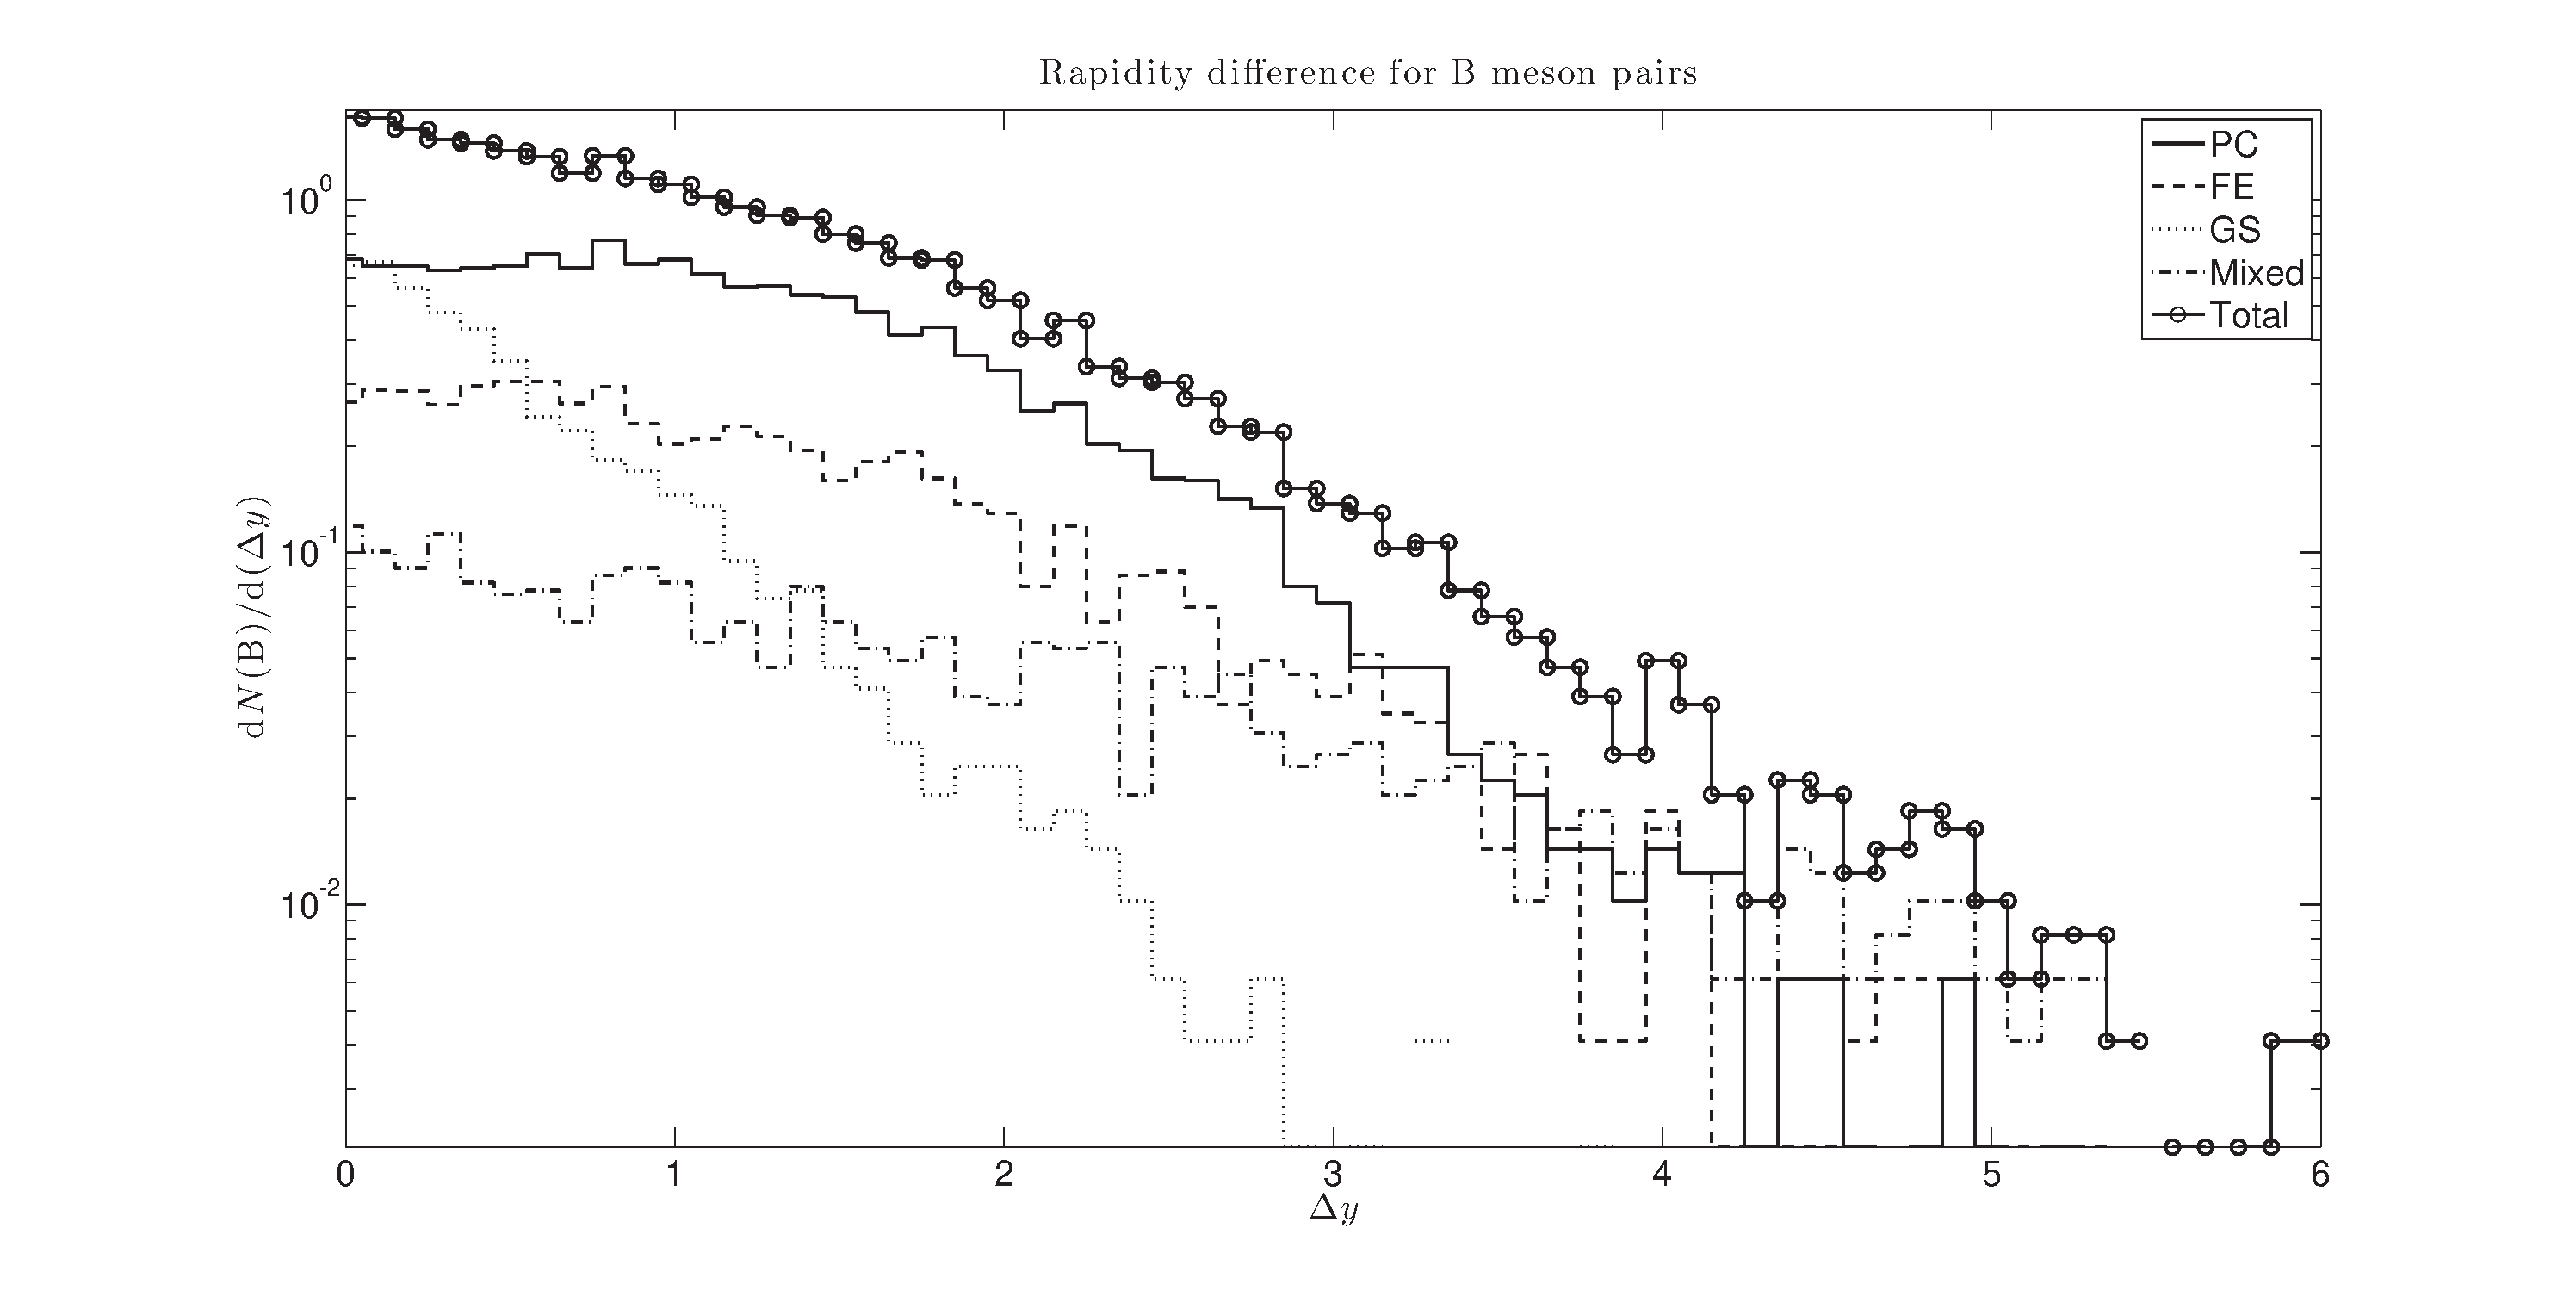
\includegraphics[width=15cm]{BBYOp1}
\label{fig:BBYOp1}
\end{figure}

\begin{figure}[!h]
\centering
\caption[[Rapidez relativa de pares de mesones $\B$. Cuatro opciones de \textsc{Pythia}.]{Rapidez relativa de pares de mesones $\B$ usando la opciones de \textsc{Pythia}:  1 (sólida), 2 (líneas), 3 (puntos) y 4 (líneas y puntos).}
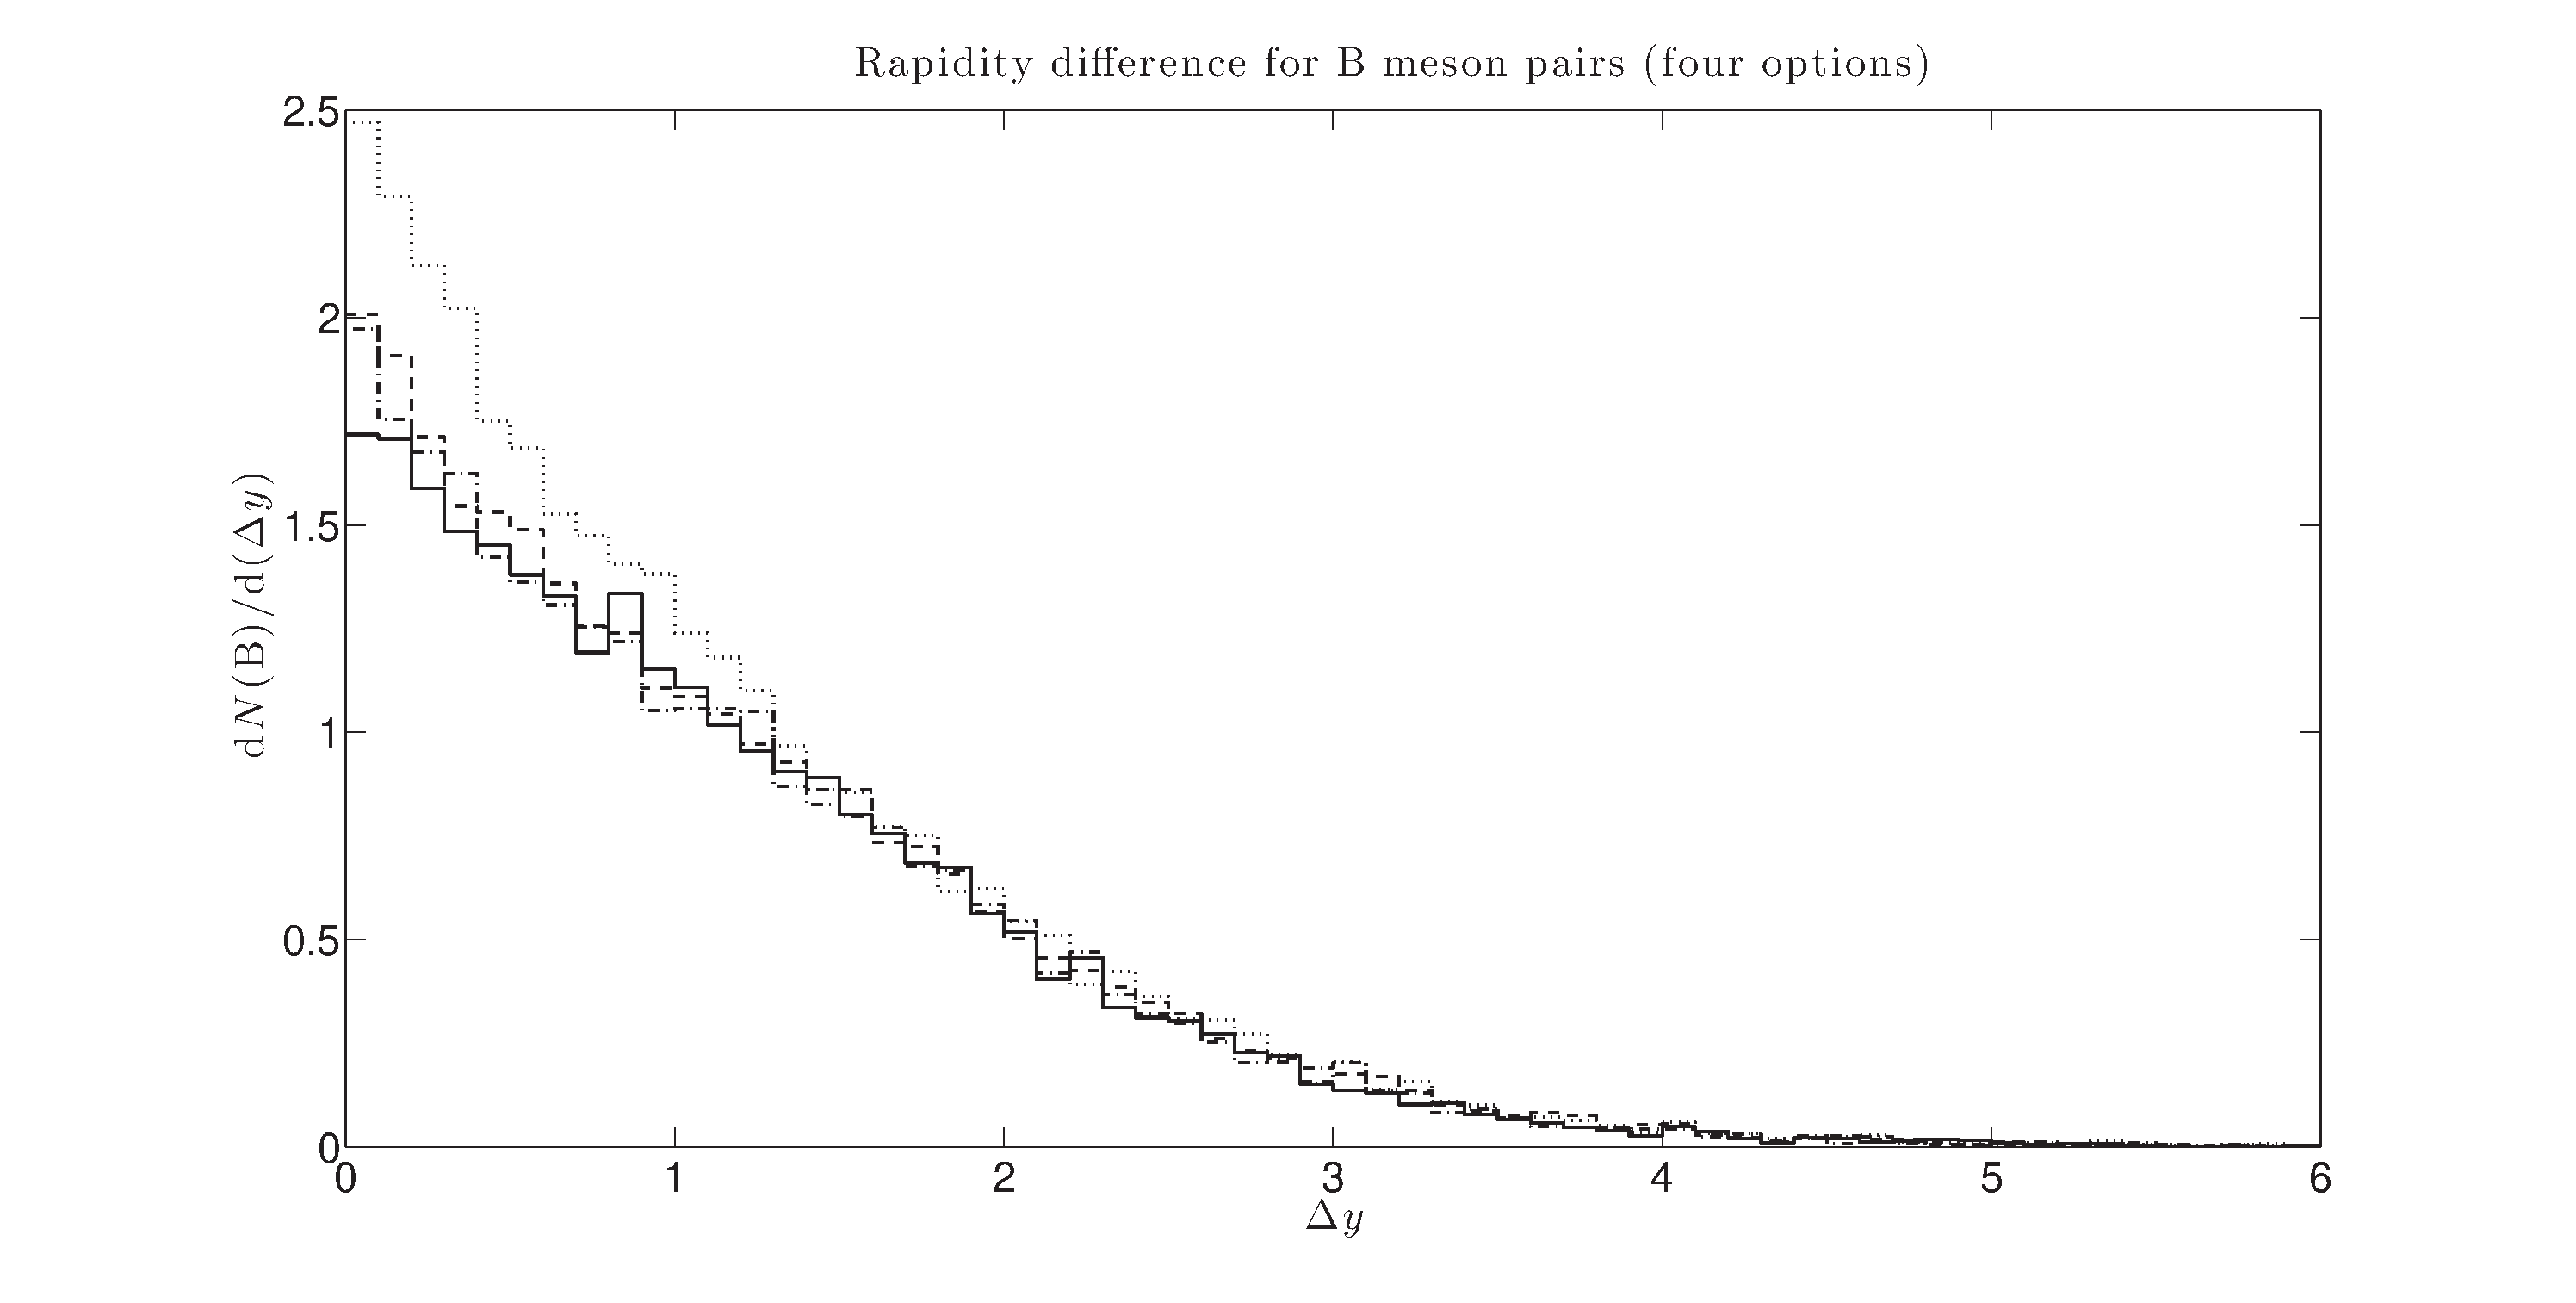
\includegraphics[width=15cm]{BBY4Op}
\label{fig:BBY4Op}
\end{figure}

Diferencias bajas en rapidez significan que las partículas en los pares están cercanas en ``distancia polar'', al mismo tiempo que un $\Delta y$ alto significa una separación polar alta. En principio, los quarks provenientes de PC son producidos con una diferencia de rapidez muy pequeña, pero los efectos cinemáticos de la lluvia de partones abren esta separación y los correspondientes mesones contribuyen significativamente en valores medianos y bajos de $\Delta y$.

La contribución de FE es menos importante que la proveniente de PC. La producción por excitación de sabor cae por debajo de GS únicamente a diferencias de rapidez bajas.

El cambio en las opciones es entonces apreciable a valores bajos de $\Delta y$, mientras que en la región media y en la cola final el comportamiento es similar en las cuatro opciones.

\subsection{Distancias $R$}

La cantidad $R$ contiene información de las dos variables estudiadas anteriormente. En cierto sentido, al dar valores de $\Delta y$ y $\Delta \varphi$ de un par de mesones, se tiene una descripción completa (Lorentz invariante ante boosts en $z$) de la distribución angular del par. En el plano $y - \varphi$ la distancia (también invarinte) $R=\sqrt{(\Delta y)^2 + (\Delta \varphi)^2}$ es útil para agrupar los pares con sus ``vecinos'' angulares. Para definir un \textit{jet de partículas} se usa típicamente la distancia $R$ para agrupar hadrones cercanos.

La figura \ref{fig:BBROp1} muestra el comportamiento de cada fuente, más la producción total de mesones $\B$ para la opción 1.
\begin{figure}[!h]
\centering
\caption[Distancia $R$ de pares de mesones $\B$. Opción por feceto de \textsc{Pythia}.]{ Distancias $R$ de pares de mesones $\B$ usando la opción por defecto de \textsc{Pythia}, incluyendo las cuatro fuentes de producción.}
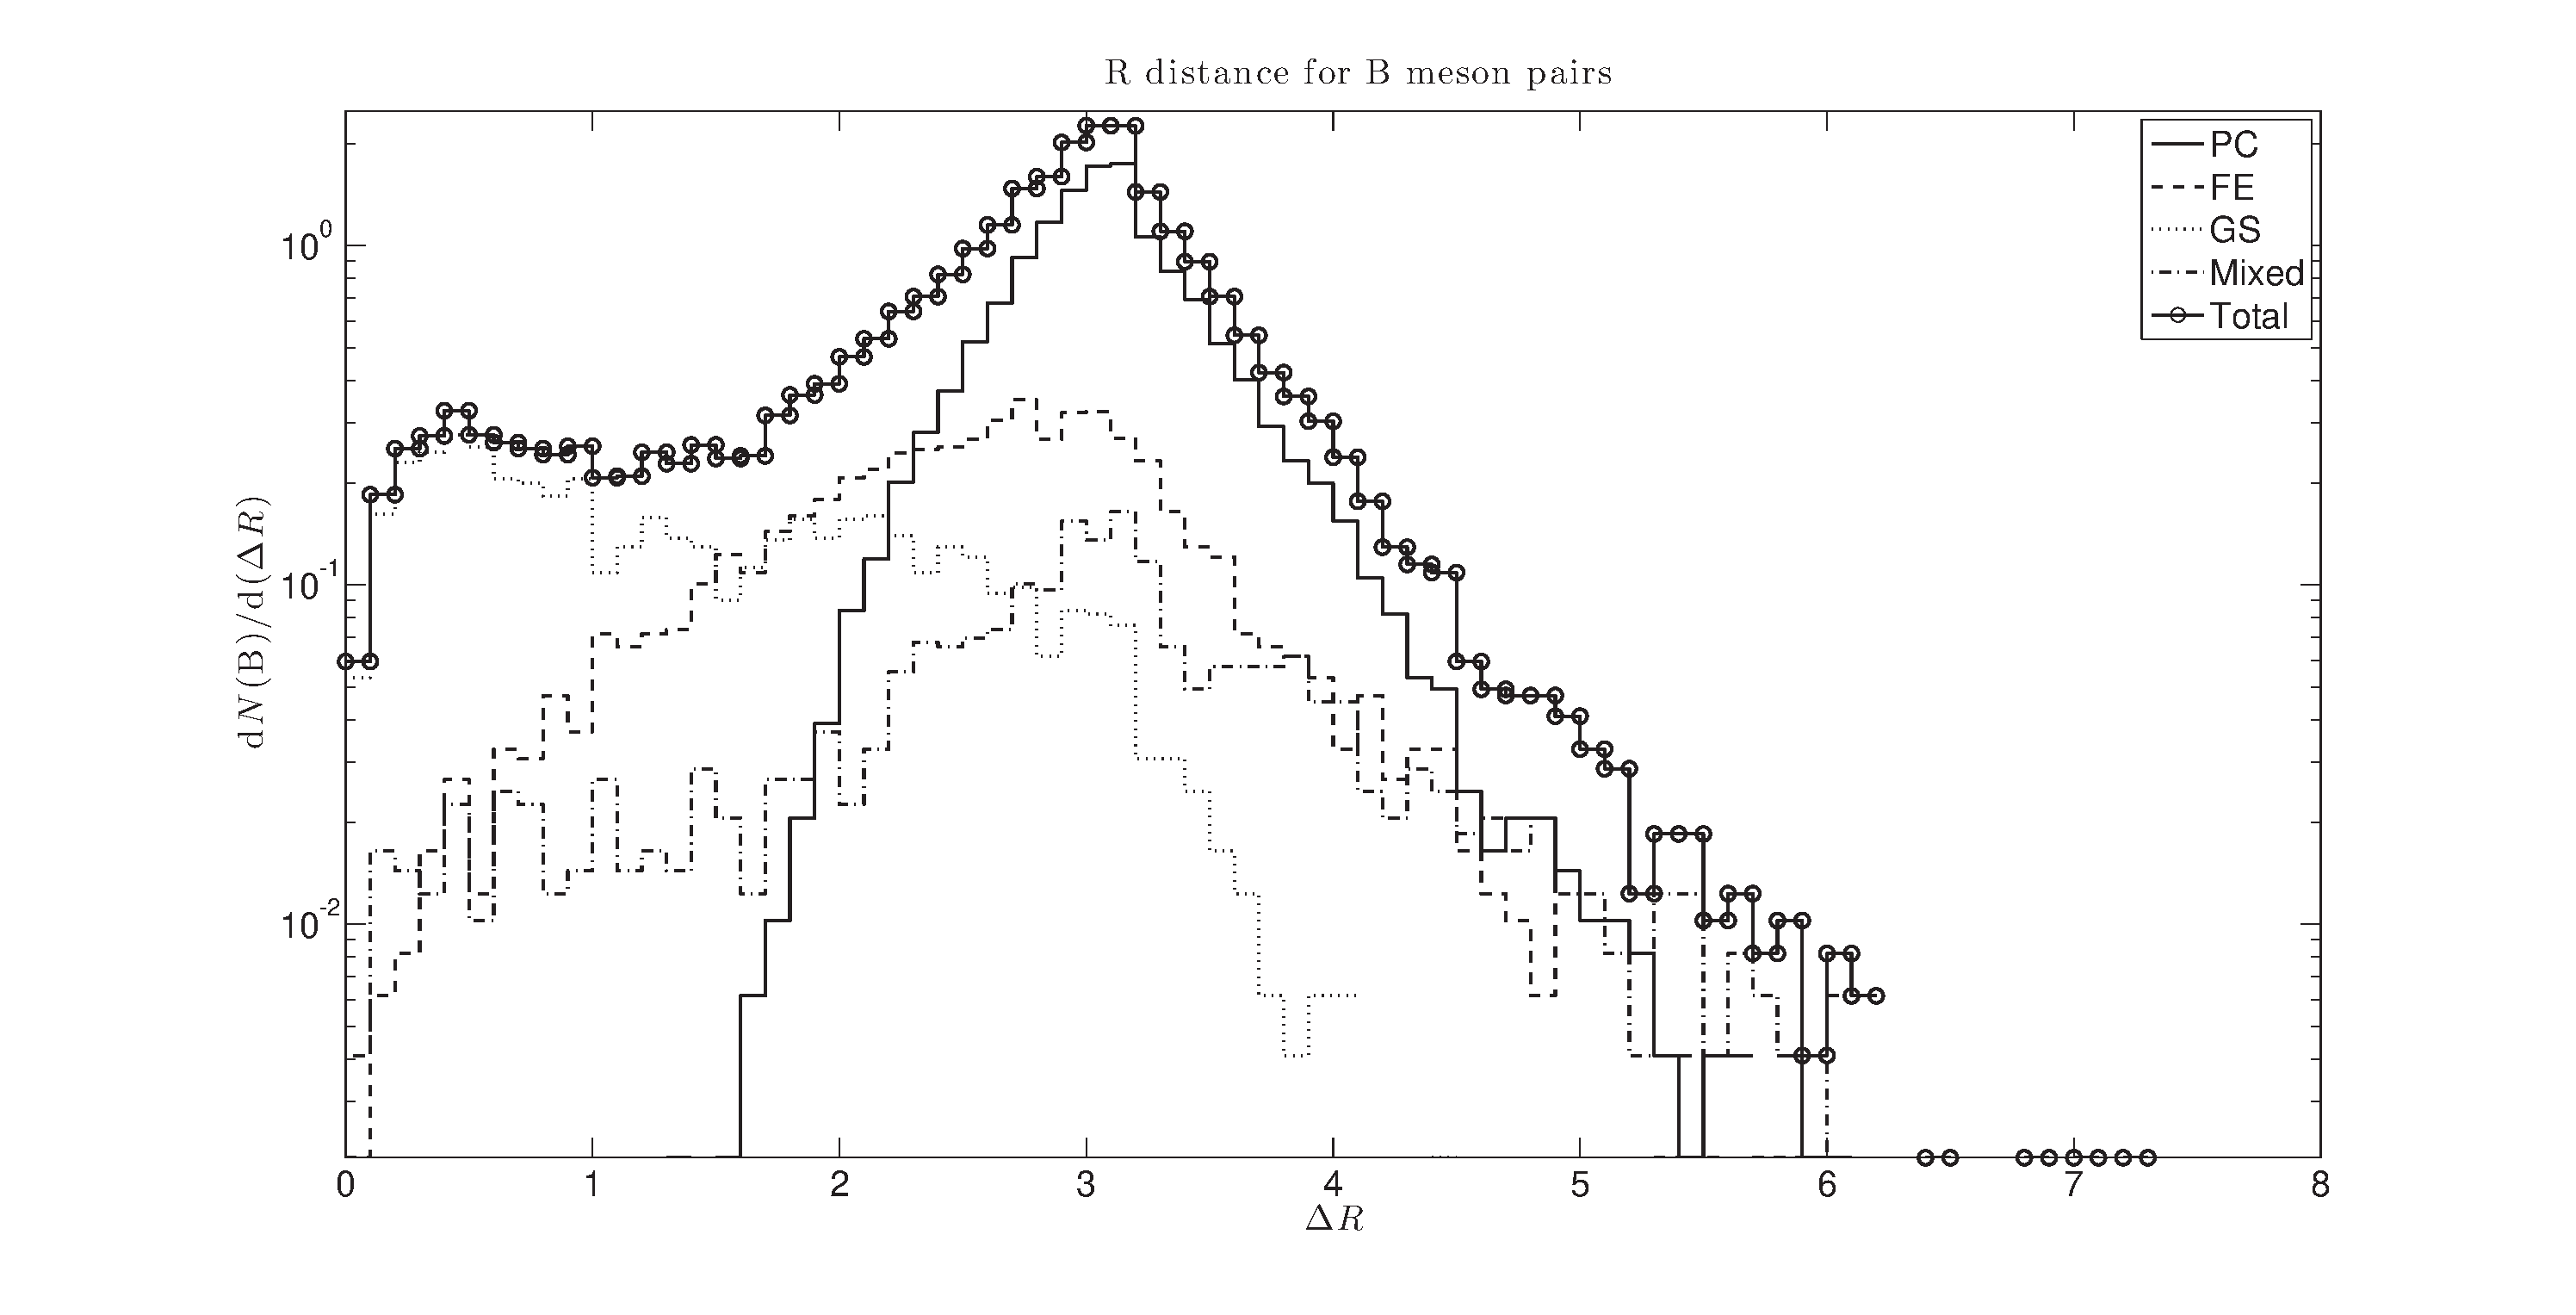
\includegraphics[width=15cm]{BBROp1}
\label{fig:BBROp1}
\end{figure}
Debido a la contribución relevante de PC a ángulos azimutales de abertura grandes, el pico principal de la distancia $R$ es cercano al valor de $\pi$. La excitación de sabor también presenta un crecimiento cerca de ese valor, aunque es menos significativo. Los mesones producidos en GS están usualmente cercanos tanto en $y$ como en $\varphi$, así que los pares clasificados como ramificación de un gluón serán probablemente agrupados en el mismo jet.
\begin{figure}[!h]
\centering
\caption[Distancia $R$ de pares de mesones $\B$. Cuatro opciones de \textsc{Pythia}.]{Distancias $R$ de pares de mesones $\B$ usando las opciones  de \textsc{Pythia}:  1 (sólida), 2 (líneas), 3 (puntos) y 4 (líneas y puntos).}
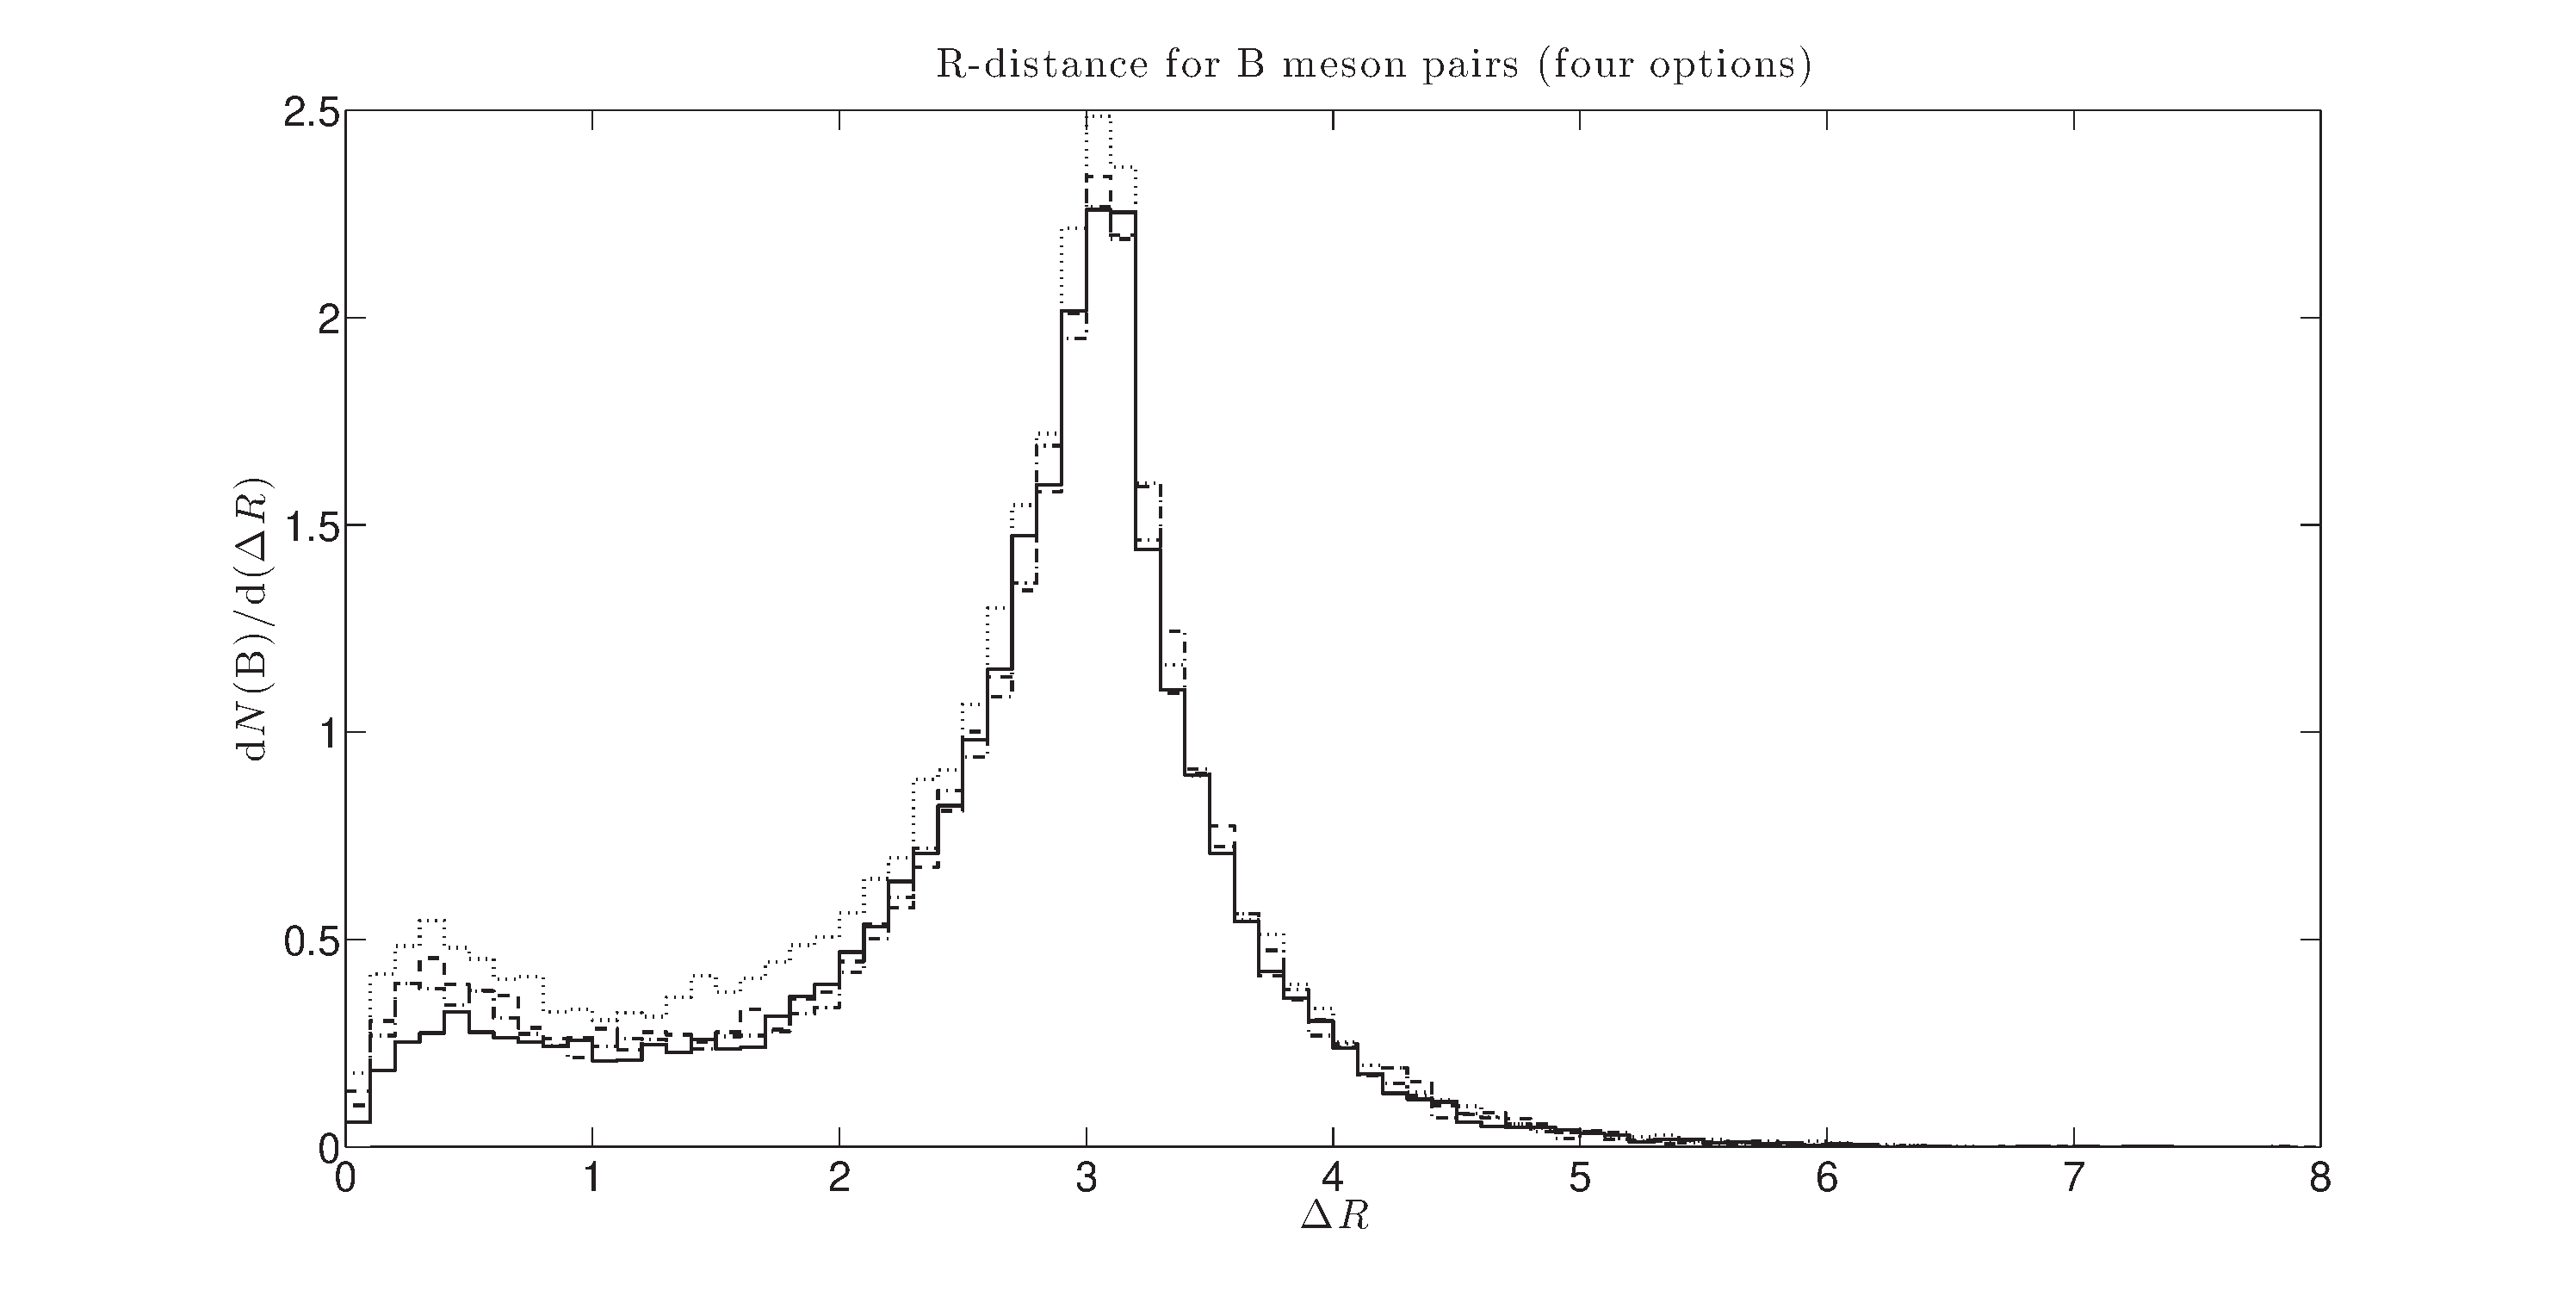
\includegraphics[width=15cm]{BBR4Op}
\label{fig:BBR4Op}
\end{figure}

Debido a que $R$ combina la información de la rapidez relativa y la abertura angular, se espera un aumento respectivo en cada una de las opciones a distancias pequeñas, que se muestra en la figura \ref{fig:BBR4Op}.

Datos experimentales sobre las correlaciones angulares de bottom pueden ser conseguidas en \cite{Khachatryan:2011wq} y \cite{ATLAS:2011ac}. Los análisis hechos ahí están incluidos en un conjunto de rutinas de validación de Rivet \cite{Buckley:2010ar}. La integración entre análisis de \textsc{Pythia} y Rivet, y la producción de datos a partir de esta, fue una maquinaria considerada para este trabajo, aunque no se logró implementar completamente debido a restricciones en el tiempo. El estudio de colisiones hadrónicas puede ser llevado a cabo también para diferentes PDFs, para observar el impacto en los mecanismos de producción y luego comparar con datos experimentales.

Existen también estudios sobre la producción de quarks $\b$ en el Tevatron (colisiones $\p\pbar$ a 2000 GeV), un ejemplo de estos es \cite{vallecorsa}.
